
% Default to the notebook output style

    


% Inherit from the specified cell style.




    
\documentclass[11pt]{article}

    
    
    \usepackage[T1]{fontenc}
    % Nicer default font (+ math font) than Computer Modern for most use cases
    \usepackage{mathpazo}

    % Basic figure setup, for now with no caption control since it's done
    % automatically by Pandoc (which extracts ![](path) syntax from Markdown).
    \usepackage{graphicx}
    % We will generate all images so they have a width \maxwidth. This means
    % that they will get their normal width if they fit onto the page, but
    % are scaled down if they would overflow the margins.
    \makeatletter
    \def\maxwidth{\ifdim\Gin@nat@width>\linewidth\linewidth
    \else\Gin@nat@width\fi}
    \makeatother
    \let\Oldincludegraphics\includegraphics
    % Set max figure width to be 80% of text width, for now hardcoded.
    \renewcommand{\includegraphics}[1]{\Oldincludegraphics[width=.8\maxwidth]{#1}}
    % Ensure that by default, figures have no caption (until we provide a
    % proper Figure object with a Caption API and a way to capture that
    % in the conversion process - todo).
    \usepackage{caption}
    \DeclareCaptionLabelFormat{nolabel}{}
    \captionsetup{labelformat=nolabel}

    \usepackage{adjustbox} % Used to constrain images to a maximum size 
    \usepackage{xcolor} % Allow colors to be defined
    \usepackage{enumerate} % Needed for markdown enumerations to work
    \usepackage{geometry} % Used to adjust the document margins
    \usepackage{amsmath} % Equations
    \usepackage{amssymb} % Equations
    \usepackage{textcomp} % defines textquotesingle
    % Hack from http://tex.stackexchange.com/a/47451/13684:
    \AtBeginDocument{%
        \def\PYZsq{\textquotesingle}% Upright quotes in Pygmentized code
    }
    \usepackage{upquote} % Upright quotes for verbatim code
    \usepackage{eurosym} % defines \euro
    \usepackage[mathletters]{ucs} % Extended unicode (utf-8) support
    \usepackage[utf8x]{inputenc} % Allow utf-8 characters in the tex document
    \usepackage{fancyvrb} % verbatim replacement that allows latex
    \usepackage{grffile} % extends the file name processing of package graphics 
                         % to support a larger range 
    % The hyperref package gives us a pdf with properly built
    % internal navigation ('pdf bookmarks' for the table of contents,
    % internal cross-reference links, web links for URLs, etc.)
    \usepackage{hyperref}
    \usepackage{longtable} % longtable support required by pandoc >1.10
    \usepackage{booktabs}  % table support for pandoc > 1.12.2
    \usepackage[inline]{enumitem} % IRkernel/repr support (it uses the enumerate* environment)
    \usepackage[normalem]{ulem} % ulem is needed to support strikethroughs (\sout)
                                % normalem makes italics be italics, not underlines
    

    
    
    % Colors for the hyperref package
    \definecolor{urlcolor}{rgb}{0,.145,.698}
    \definecolor{linkcolor}{rgb}{.71,0.21,0.01}
    \definecolor{citecolor}{rgb}{.12,.54,.11}

    % ANSI colors
    \definecolor{ansi-black}{HTML}{3E424D}
    \definecolor{ansi-black-intense}{HTML}{282C36}
    \definecolor{ansi-red}{HTML}{E75C58}
    \definecolor{ansi-red-intense}{HTML}{B22B31}
    \definecolor{ansi-green}{HTML}{00A250}
    \definecolor{ansi-green-intense}{HTML}{007427}
    \definecolor{ansi-yellow}{HTML}{DDB62B}
    \definecolor{ansi-yellow-intense}{HTML}{B27D12}
    \definecolor{ansi-blue}{HTML}{208FFB}
    \definecolor{ansi-blue-intense}{HTML}{0065CA}
    \definecolor{ansi-magenta}{HTML}{D160C4}
    \definecolor{ansi-magenta-intense}{HTML}{A03196}
    \definecolor{ansi-cyan}{HTML}{60C6C8}
    \definecolor{ansi-cyan-intense}{HTML}{258F8F}
    \definecolor{ansi-white}{HTML}{C5C1B4}
    \definecolor{ansi-white-intense}{HTML}{A1A6B2}

    % commands and environments needed by pandoc snippets
    % extracted from the output of `pandoc -s`
    \providecommand{\tightlist}{%
      \setlength{\itemsep}{0pt}\setlength{\parskip}{0pt}}
    \DefineVerbatimEnvironment{Highlighting}{Verbatim}{commandchars=\\\{\}}
    % Add ',fontsize=\small' for more characters per line
    \newenvironment{Shaded}{}{}
    \newcommand{\KeywordTok}[1]{\textcolor[rgb]{0.00,0.44,0.13}{\textbf{{#1}}}}
    \newcommand{\DataTypeTok}[1]{\textcolor[rgb]{0.56,0.13,0.00}{{#1}}}
    \newcommand{\DecValTok}[1]{\textcolor[rgb]{0.25,0.63,0.44}{{#1}}}
    \newcommand{\BaseNTok}[1]{\textcolor[rgb]{0.25,0.63,0.44}{{#1}}}
    \newcommand{\FloatTok}[1]{\textcolor[rgb]{0.25,0.63,0.44}{{#1}}}
    \newcommand{\CharTok}[1]{\textcolor[rgb]{0.25,0.44,0.63}{{#1}}}
    \newcommand{\StringTok}[1]{\textcolor[rgb]{0.25,0.44,0.63}{{#1}}}
    \newcommand{\CommentTok}[1]{\textcolor[rgb]{0.38,0.63,0.69}{\textit{{#1}}}}
    \newcommand{\OtherTok}[1]{\textcolor[rgb]{0.00,0.44,0.13}{{#1}}}
    \newcommand{\AlertTok}[1]{\textcolor[rgb]{1.00,0.00,0.00}{\textbf{{#1}}}}
    \newcommand{\FunctionTok}[1]{\textcolor[rgb]{0.02,0.16,0.49}{{#1}}}
    \newcommand{\RegionMarkerTok}[1]{{#1}}
    \newcommand{\ErrorTok}[1]{\textcolor[rgb]{1.00,0.00,0.00}{\textbf{{#1}}}}
    \newcommand{\NormalTok}[1]{{#1}}
    
    % Additional commands for more recent versions of Pandoc
    \newcommand{\ConstantTok}[1]{\textcolor[rgb]{0.53,0.00,0.00}{{#1}}}
    \newcommand{\SpecialCharTok}[1]{\textcolor[rgb]{0.25,0.44,0.63}{{#1}}}
    \newcommand{\VerbatimStringTok}[1]{\textcolor[rgb]{0.25,0.44,0.63}{{#1}}}
    \newcommand{\SpecialStringTok}[1]{\textcolor[rgb]{0.73,0.40,0.53}{{#1}}}
    \newcommand{\ImportTok}[1]{{#1}}
    \newcommand{\DocumentationTok}[1]{\textcolor[rgb]{0.73,0.13,0.13}{\textit{{#1}}}}
    \newcommand{\AnnotationTok}[1]{\textcolor[rgb]{0.38,0.63,0.69}{\textbf{\textit{{#1}}}}}
    \newcommand{\CommentVarTok}[1]{\textcolor[rgb]{0.38,0.63,0.69}{\textbf{\textit{{#1}}}}}
    \newcommand{\VariableTok}[1]{\textcolor[rgb]{0.10,0.09,0.49}{{#1}}}
    \newcommand{\ControlFlowTok}[1]{\textcolor[rgb]{0.00,0.44,0.13}{\textbf{{#1}}}}
    \newcommand{\OperatorTok}[1]{\textcolor[rgb]{0.40,0.40,0.40}{{#1}}}
    \newcommand{\BuiltInTok}[1]{{#1}}
    \newcommand{\ExtensionTok}[1]{{#1}}
    \newcommand{\PreprocessorTok}[1]{\textcolor[rgb]{0.74,0.48,0.00}{{#1}}}
    \newcommand{\AttributeTok}[1]{\textcolor[rgb]{0.49,0.56,0.16}{{#1}}}
    \newcommand{\InformationTok}[1]{\textcolor[rgb]{0.38,0.63,0.69}{\textbf{\textit{{#1}}}}}
    \newcommand{\WarningTok}[1]{\textcolor[rgb]{0.38,0.63,0.69}{\textbf{\textit{{#1}}}}}
    
    
    % Define a nice break command that doesn't care if a line doesn't already
    % exist.
    \def\br{\hspace*{\fill} \\* }
    % Math Jax compatability definitions
    \def\gt{>}
    \def\lt{<}
    % Document parameters
    \title{hw2\_regression\_classification\_webscraping\_v2}
    
    
    

    % Pygments definitions
    
\makeatletter
\def\PY@reset{\let\PY@it=\relax \let\PY@bf=\relax%
    \let\PY@ul=\relax \let\PY@tc=\relax%
    \let\PY@bc=\relax \let\PY@ff=\relax}
\def\PY@tok#1{\csname PY@tok@#1\endcsname}
\def\PY@toks#1+{\ifx\relax#1\empty\else%
    \PY@tok{#1}\expandafter\PY@toks\fi}
\def\PY@do#1{\PY@bc{\PY@tc{\PY@ul{%
    \PY@it{\PY@bf{\PY@ff{#1}}}}}}}
\def\PY#1#2{\PY@reset\PY@toks#1+\relax+\PY@do{#2}}

\expandafter\def\csname PY@tok@w\endcsname{\def\PY@tc##1{\textcolor[rgb]{0.73,0.73,0.73}{##1}}}
\expandafter\def\csname PY@tok@c\endcsname{\let\PY@it=\textit\def\PY@tc##1{\textcolor[rgb]{0.25,0.50,0.50}{##1}}}
\expandafter\def\csname PY@tok@cp\endcsname{\def\PY@tc##1{\textcolor[rgb]{0.74,0.48,0.00}{##1}}}
\expandafter\def\csname PY@tok@k\endcsname{\let\PY@bf=\textbf\def\PY@tc##1{\textcolor[rgb]{0.00,0.50,0.00}{##1}}}
\expandafter\def\csname PY@tok@kp\endcsname{\def\PY@tc##1{\textcolor[rgb]{0.00,0.50,0.00}{##1}}}
\expandafter\def\csname PY@tok@kt\endcsname{\def\PY@tc##1{\textcolor[rgb]{0.69,0.00,0.25}{##1}}}
\expandafter\def\csname PY@tok@o\endcsname{\def\PY@tc##1{\textcolor[rgb]{0.40,0.40,0.40}{##1}}}
\expandafter\def\csname PY@tok@ow\endcsname{\let\PY@bf=\textbf\def\PY@tc##1{\textcolor[rgb]{0.67,0.13,1.00}{##1}}}
\expandafter\def\csname PY@tok@nb\endcsname{\def\PY@tc##1{\textcolor[rgb]{0.00,0.50,0.00}{##1}}}
\expandafter\def\csname PY@tok@nf\endcsname{\def\PY@tc##1{\textcolor[rgb]{0.00,0.00,1.00}{##1}}}
\expandafter\def\csname PY@tok@nc\endcsname{\let\PY@bf=\textbf\def\PY@tc##1{\textcolor[rgb]{0.00,0.00,1.00}{##1}}}
\expandafter\def\csname PY@tok@nn\endcsname{\let\PY@bf=\textbf\def\PY@tc##1{\textcolor[rgb]{0.00,0.00,1.00}{##1}}}
\expandafter\def\csname PY@tok@ne\endcsname{\let\PY@bf=\textbf\def\PY@tc##1{\textcolor[rgb]{0.82,0.25,0.23}{##1}}}
\expandafter\def\csname PY@tok@nv\endcsname{\def\PY@tc##1{\textcolor[rgb]{0.10,0.09,0.49}{##1}}}
\expandafter\def\csname PY@tok@no\endcsname{\def\PY@tc##1{\textcolor[rgb]{0.53,0.00,0.00}{##1}}}
\expandafter\def\csname PY@tok@nl\endcsname{\def\PY@tc##1{\textcolor[rgb]{0.63,0.63,0.00}{##1}}}
\expandafter\def\csname PY@tok@ni\endcsname{\let\PY@bf=\textbf\def\PY@tc##1{\textcolor[rgb]{0.60,0.60,0.60}{##1}}}
\expandafter\def\csname PY@tok@na\endcsname{\def\PY@tc##1{\textcolor[rgb]{0.49,0.56,0.16}{##1}}}
\expandafter\def\csname PY@tok@nt\endcsname{\let\PY@bf=\textbf\def\PY@tc##1{\textcolor[rgb]{0.00,0.50,0.00}{##1}}}
\expandafter\def\csname PY@tok@nd\endcsname{\def\PY@tc##1{\textcolor[rgb]{0.67,0.13,1.00}{##1}}}
\expandafter\def\csname PY@tok@s\endcsname{\def\PY@tc##1{\textcolor[rgb]{0.73,0.13,0.13}{##1}}}
\expandafter\def\csname PY@tok@sd\endcsname{\let\PY@it=\textit\def\PY@tc##1{\textcolor[rgb]{0.73,0.13,0.13}{##1}}}
\expandafter\def\csname PY@tok@si\endcsname{\let\PY@bf=\textbf\def\PY@tc##1{\textcolor[rgb]{0.73,0.40,0.53}{##1}}}
\expandafter\def\csname PY@tok@se\endcsname{\let\PY@bf=\textbf\def\PY@tc##1{\textcolor[rgb]{0.73,0.40,0.13}{##1}}}
\expandafter\def\csname PY@tok@sr\endcsname{\def\PY@tc##1{\textcolor[rgb]{0.73,0.40,0.53}{##1}}}
\expandafter\def\csname PY@tok@ss\endcsname{\def\PY@tc##1{\textcolor[rgb]{0.10,0.09,0.49}{##1}}}
\expandafter\def\csname PY@tok@sx\endcsname{\def\PY@tc##1{\textcolor[rgb]{0.00,0.50,0.00}{##1}}}
\expandafter\def\csname PY@tok@m\endcsname{\def\PY@tc##1{\textcolor[rgb]{0.40,0.40,0.40}{##1}}}
\expandafter\def\csname PY@tok@gh\endcsname{\let\PY@bf=\textbf\def\PY@tc##1{\textcolor[rgb]{0.00,0.00,0.50}{##1}}}
\expandafter\def\csname PY@tok@gu\endcsname{\let\PY@bf=\textbf\def\PY@tc##1{\textcolor[rgb]{0.50,0.00,0.50}{##1}}}
\expandafter\def\csname PY@tok@gd\endcsname{\def\PY@tc##1{\textcolor[rgb]{0.63,0.00,0.00}{##1}}}
\expandafter\def\csname PY@tok@gi\endcsname{\def\PY@tc##1{\textcolor[rgb]{0.00,0.63,0.00}{##1}}}
\expandafter\def\csname PY@tok@gr\endcsname{\def\PY@tc##1{\textcolor[rgb]{1.00,0.00,0.00}{##1}}}
\expandafter\def\csname PY@tok@ge\endcsname{\let\PY@it=\textit}
\expandafter\def\csname PY@tok@gs\endcsname{\let\PY@bf=\textbf}
\expandafter\def\csname PY@tok@gp\endcsname{\let\PY@bf=\textbf\def\PY@tc##1{\textcolor[rgb]{0.00,0.00,0.50}{##1}}}
\expandafter\def\csname PY@tok@go\endcsname{\def\PY@tc##1{\textcolor[rgb]{0.53,0.53,0.53}{##1}}}
\expandafter\def\csname PY@tok@gt\endcsname{\def\PY@tc##1{\textcolor[rgb]{0.00,0.27,0.87}{##1}}}
\expandafter\def\csname PY@tok@err\endcsname{\def\PY@bc##1{\setlength{\fboxsep}{0pt}\fcolorbox[rgb]{1.00,0.00,0.00}{1,1,1}{\strut ##1}}}
\expandafter\def\csname PY@tok@kc\endcsname{\let\PY@bf=\textbf\def\PY@tc##1{\textcolor[rgb]{0.00,0.50,0.00}{##1}}}
\expandafter\def\csname PY@tok@kd\endcsname{\let\PY@bf=\textbf\def\PY@tc##1{\textcolor[rgb]{0.00,0.50,0.00}{##1}}}
\expandafter\def\csname PY@tok@kn\endcsname{\let\PY@bf=\textbf\def\PY@tc##1{\textcolor[rgb]{0.00,0.50,0.00}{##1}}}
\expandafter\def\csname PY@tok@kr\endcsname{\let\PY@bf=\textbf\def\PY@tc##1{\textcolor[rgb]{0.00,0.50,0.00}{##1}}}
\expandafter\def\csname PY@tok@bp\endcsname{\def\PY@tc##1{\textcolor[rgb]{0.00,0.50,0.00}{##1}}}
\expandafter\def\csname PY@tok@fm\endcsname{\def\PY@tc##1{\textcolor[rgb]{0.00,0.00,1.00}{##1}}}
\expandafter\def\csname PY@tok@vc\endcsname{\def\PY@tc##1{\textcolor[rgb]{0.10,0.09,0.49}{##1}}}
\expandafter\def\csname PY@tok@vg\endcsname{\def\PY@tc##1{\textcolor[rgb]{0.10,0.09,0.49}{##1}}}
\expandafter\def\csname PY@tok@vi\endcsname{\def\PY@tc##1{\textcolor[rgb]{0.10,0.09,0.49}{##1}}}
\expandafter\def\csname PY@tok@vm\endcsname{\def\PY@tc##1{\textcolor[rgb]{0.10,0.09,0.49}{##1}}}
\expandafter\def\csname PY@tok@sa\endcsname{\def\PY@tc##1{\textcolor[rgb]{0.73,0.13,0.13}{##1}}}
\expandafter\def\csname PY@tok@sb\endcsname{\def\PY@tc##1{\textcolor[rgb]{0.73,0.13,0.13}{##1}}}
\expandafter\def\csname PY@tok@sc\endcsname{\def\PY@tc##1{\textcolor[rgb]{0.73,0.13,0.13}{##1}}}
\expandafter\def\csname PY@tok@dl\endcsname{\def\PY@tc##1{\textcolor[rgb]{0.73,0.13,0.13}{##1}}}
\expandafter\def\csname PY@tok@s2\endcsname{\def\PY@tc##1{\textcolor[rgb]{0.73,0.13,0.13}{##1}}}
\expandafter\def\csname PY@tok@sh\endcsname{\def\PY@tc##1{\textcolor[rgb]{0.73,0.13,0.13}{##1}}}
\expandafter\def\csname PY@tok@s1\endcsname{\def\PY@tc##1{\textcolor[rgb]{0.73,0.13,0.13}{##1}}}
\expandafter\def\csname PY@tok@mb\endcsname{\def\PY@tc##1{\textcolor[rgb]{0.40,0.40,0.40}{##1}}}
\expandafter\def\csname PY@tok@mf\endcsname{\def\PY@tc##1{\textcolor[rgb]{0.40,0.40,0.40}{##1}}}
\expandafter\def\csname PY@tok@mh\endcsname{\def\PY@tc##1{\textcolor[rgb]{0.40,0.40,0.40}{##1}}}
\expandafter\def\csname PY@tok@mi\endcsname{\def\PY@tc##1{\textcolor[rgb]{0.40,0.40,0.40}{##1}}}
\expandafter\def\csname PY@tok@il\endcsname{\def\PY@tc##1{\textcolor[rgb]{0.40,0.40,0.40}{##1}}}
\expandafter\def\csname PY@tok@mo\endcsname{\def\PY@tc##1{\textcolor[rgb]{0.40,0.40,0.40}{##1}}}
\expandafter\def\csname PY@tok@ch\endcsname{\let\PY@it=\textit\def\PY@tc##1{\textcolor[rgb]{0.25,0.50,0.50}{##1}}}
\expandafter\def\csname PY@tok@cm\endcsname{\let\PY@it=\textit\def\PY@tc##1{\textcolor[rgb]{0.25,0.50,0.50}{##1}}}
\expandafter\def\csname PY@tok@cpf\endcsname{\let\PY@it=\textit\def\PY@tc##1{\textcolor[rgb]{0.25,0.50,0.50}{##1}}}
\expandafter\def\csname PY@tok@c1\endcsname{\let\PY@it=\textit\def\PY@tc##1{\textcolor[rgb]{0.25,0.50,0.50}{##1}}}
\expandafter\def\csname PY@tok@cs\endcsname{\let\PY@it=\textit\def\PY@tc##1{\textcolor[rgb]{0.25,0.50,0.50}{##1}}}

\def\PYZbs{\char`\\}
\def\PYZus{\char`\_}
\def\PYZob{\char`\{}
\def\PYZcb{\char`\}}
\def\PYZca{\char`\^}
\def\PYZam{\char`\&}
\def\PYZlt{\char`\<}
\def\PYZgt{\char`\>}
\def\PYZsh{\char`\#}
\def\PYZpc{\char`\%}
\def\PYZdl{\char`\$}
\def\PYZhy{\char`\-}
\def\PYZsq{\char`\'}
\def\PYZdq{\char`\"}
\def\PYZti{\char`\~}
% for compatibility with earlier versions
\def\PYZat{@}
\def\PYZlb{[}
\def\PYZrb{]}
\makeatother


    % Exact colors from NB
    \definecolor{incolor}{rgb}{0.0, 0.0, 0.5}
    \definecolor{outcolor}{rgb}{0.545, 0.0, 0.0}



    
    % Prevent overflowing lines due to hard-to-break entities
    \sloppy 
    % Setup hyperref package
    \hypersetup{
      breaklinks=true,  % so long urls are correctly broken across lines
      colorlinks=true,
      urlcolor=urlcolor,
      linkcolor=linkcolor,
      citecolor=citecolor,
      }
    % Slightly bigger margins than the latex defaults
    
    \geometry{verbose,tmargin=1in,bmargin=1in,lmargin=1in,rmargin=1in}
    
    

    \begin{document}
    
    
    \maketitle
    
    

    
    \section{Data-X Spring 2018: Homework
02}\label{data-x-spring-2018-homework-02}

\subsubsection{Regression, Classification,
Webscraping}\label{regression-classification-webscraping}

\textbf{Authors:} Sana Iqbal (Part 1, 2, 3), Alexander Fred-Ojala (Extra
Credit)

In this homework, you will do some exercises with
prediction-classification, regression and web-scraping.

    \subsection{Part 1}\label{part-1}

    \subsubsection{Data:}\label{data}

\textbf{Data Source}: Data file is uploaded to bCourses and is named:
\textbf{Energy.csv}

The dataset was created by Angeliki Xifara ( Civil/Structural Engineer)
and was processed by Athanasios Tsanas, Oxford Centre for Industrial and
Applied Mathematics, University of Oxford, UK).

\textbf{Data Description}:

The dataset contains eight attributes of a building (or features,
denoted by X1...X8) and response being the heating load on the building,
y1.

\begin{itemize}
\tightlist
\item
  X1 Relative Compactness
\item
  X2 Surface Area
\item
  X3 Wall Area
\item
  X4 Roof Area
\item
  X5 Overall Height
\item
  X6 Orientation
\item
  X7 Glazing Area
\item
  X8 Glazing Area Distribution
\item
  y1 Heating Load
\end{itemize}

    \paragraph{Q1:Read the data file in python. Describe data features in
terms of type, distribution range and mean values. Plot feature
distributions.This step should give you clues about data
sufficiency.}\label{q1read-the-data-file-in-python.-describe-data-features-in-terms-of-type-distribution-range-and-mean-values.-plot-feature-distributions.this-step-should-give-you-clues-about-data-sufficiency.}

    \begin{Verbatim}[commandchars=\\\{\}]
{\color{incolor}In [{\color{incolor} }]:} \PY{c+c1}{\PYZsh{} Import Package}
        \PY{k+kn}{import} \PY{n+nn}{numpy} \PY{k}{as} \PY{n+nn}{np}
        \PY{k+kn}{import} \PY{n+nn}{pandas} \PY{k}{as} \PY{n+nn}{pd}
        \PY{k+kn}{import} \PY{n+nn}{matplotlib}\PY{n+nn}{.}\PY{n+nn}{pyplot} \PY{k}{as} \PY{n+nn}{plt}
        
        \PY{k+kn}{from} \PY{n+nn}{sklearn}\PY{n+nn}{.}\PY{n+nn}{utils} \PY{k}{import} \PY{n}{shuffle}
        \PY{k+kn}{from} \PY{n+nn}{sklearn}\PY{n+nn}{.}\PY{n+nn}{model\PYZus{}selection} \PY{k}{import} \PY{n}{train\PYZus{}test\PYZus{}split}
        
        \PY{k+kn}{from} \PY{n+nn}{sklearn}\PY{n+nn}{.}\PY{n+nn}{linear\PYZus{}model} \PY{k}{import} \PY{n}{LinearRegression}
        \PY{k+kn}{from} \PY{n+nn}{sklearn}\PY{n+nn}{.}\PY{n+nn}{linear\PYZus{}model} \PY{k}{import} \PY{n}{LogisticRegression}
        \PY{k+kn}{from} \PY{n+nn}{sklearn}\PY{n+nn}{.}\PY{n+nn}{svm} \PY{k}{import} \PY{n}{SVC}\PY{p}{,} \PY{n}{LinearSVC}
        \PY{k+kn}{from} \PY{n+nn}{sklearn}\PY{n+nn}{.}\PY{n+nn}{linear\PYZus{}model} \PY{k}{import} \PY{n}{Perceptron}
        \PY{k+kn}{from} \PY{n+nn}{sklearn}\PY{n+nn}{.}\PY{n+nn}{neighbors} \PY{k}{import} \PY{n}{KNeighborsClassifier}
        \PY{k+kn}{from} \PY{n+nn}{sklearn}\PY{n+nn}{.}\PY{n+nn}{ensemble} \PY{k}{import} \PY{n}{RandomForestClassifier}
        
        \PY{k+kn}{import} \PY{n+nn}{xgboost} \PY{k}{as} \PY{n+nn}{xgb}
        
        
        \PY{o}{\PYZpc{}}\PY{k}{matplotlib} inline
\end{Verbatim}


    \begin{Verbatim}[commandchars=\\\{\}]
{\color{incolor}In [{\color{incolor} }]:} \PY{c+c1}{\PYZsh{} Distribution of each variable.}
        \PY{c+c1}{\PYZsh{} Reading FileD}
        \PY{n}{df} \PY{o}{=} \PY{n}{pd}\PY{o}{.}\PY{n}{read\PYZus{}csv}\PY{p}{(}\PY{l+s+s1}{\PYZsq{}}\PY{l+s+s1}{Energy.csv}\PY{l+s+s1}{\PYZsq{}}\PY{p}{)}
\end{Verbatim}


    \begin{Verbatim}[commandchars=\\\{\}]
{\color{incolor}In [{\color{incolor} }]:} \PY{c+c1}{\PYZsh{} Describing data (General)}
        \PY{n+nb}{print}\PY{p}{(}\PY{l+s+s2}{\PYZdq{}}\PY{l+s+s2}{Describing Data in a general view...}\PY{l+s+s2}{\PYZdq{}}\PY{p}{)}
        \PY{n}{df}\PY{o}{.}\PY{n}{describe}\PY{p}{(}\PY{p}{)}
\end{Verbatim}


    \begin{Verbatim}[commandchars=\\\{\}]
{\color{incolor}In [{\color{incolor} }]:} \PY{c+c1}{\PYZsh{} Describe data features in terms of type, distribution range and mean values.}
        
        \PY{k}{def} \PY{n+nf}{nice\PYZus{}display\PYZus{}basic\PYZus{}statistics}\PY{p}{(}\PY{n}{maxi}\PY{p}{,} \PY{n}{mini}\PY{p}{,} \PY{n}{mean}\PY{p}{)}\PY{p}{:}
            \PY{l+s+sd}{\PYZdq{}\PYZdq{}\PYZdq{}}
        \PY{l+s+sd}{    Print in a nice way the data features distribution range and mean values}
        
        \PY{l+s+sd}{    Arguments:}
        \PY{l+s+sd}{        maxi \PYZhy{}\PYZhy{} python float containing the Max of the feature}
        \PY{l+s+sd}{        mini \PYZhy{}\PYZhy{} python float containing the Min of the feature}
        \PY{l+s+sd}{        mean \PYZhy{}\PYZhy{} python float containing the Mean of the feature}
        
        \PY{l+s+sd}{    \PYZdq{}\PYZdq{}\PYZdq{}}
            
            \PY{n+nb}{print}\PY{p}{(}\PY{l+s+s2}{\PYZdq{}}\PY{l+s+s2}{Max: }\PY{l+s+s2}{\PYZdq{}}\PY{p}{,} \PY{n}{maxi}\PY{p}{)}
            \PY{n+nb}{print}\PY{p}{(}\PY{l+s+s2}{\PYZdq{}}\PY{l+s+s2}{Min: }\PY{l+s+s2}{\PYZdq{}}\PY{p}{,} \PY{n}{mini}\PY{p}{)}
            \PY{n+nb}{print}\PY{p}{(}\PY{l+s+s2}{\PYZdq{}}\PY{l+s+s2}{Mean}\PY{l+s+s2}{\PYZdq{}}\PY{p}{,} \PY{n}{mean}\PY{p}{)}
                
                
        \PY{k}{def} \PY{n+nf}{nice\PYZus{}display}\PY{p}{(}\PY{n}{column\PYZus{}name}\PY{p}{,} \PY{n}{dtype}\PY{p}{,} \PY{n}{maxi}\PY{p}{,} \PY{n}{mini}\PY{p}{,} \PY{n}{mean}\PY{p}{)}\PY{p}{:}
            \PY{l+s+sd}{\PYZdq{}\PYZdq{}\PYZdq{}}
        \PY{l+s+sd}{    Print in a nice way the data features in terms of type, distribution range and mean values}
        
        \PY{l+s+sd}{    Arguments:}
        \PY{l+s+sd}{        column\PYZus{}name \PYZhy{}\PYZhy{} python string containing the name of the feature}
        \PY{l+s+sd}{        dtype \PYZhy{}\PYZhy{} python string containing the dtype of the feature}
        \PY{l+s+sd}{        maxi \PYZhy{}\PYZhy{} python float containing the Max of the feature}
        \PY{l+s+sd}{        mini \PYZhy{}\PYZhy{} python float containing the Min of the feature}
        \PY{l+s+sd}{        mean \PYZhy{}\PYZhy{} python float containing the Mean of the feature}
        \PY{l+s+sd}{        }
        \PY{l+s+sd}{    \PYZdq{}\PYZdq{}\PYZdq{}}
            
            \PY{k}{if} \PY{n}{dtype} \PY{o}{==} \PY{l+s+s2}{\PYZdq{}}\PY{l+s+s2}{float64}\PY{l+s+s2}{\PYZdq{}}\PY{p}{:}        
                \PY{n+nb}{print}\PY{p}{(}\PY{l+s+s2}{\PYZdq{}}\PY{l+s+s2}{The feature }\PY{l+s+s2}{\PYZdq{}} \PY{o}{+} \PY{n}{column\PYZus{}name} \PY{o}{+} \PY{l+s+s2}{\PYZdq{}}\PY{l+s+s2}{: }\PY{l+s+s2}{\PYZdq{}}\PY{p}{)}
                \PY{n+nb}{print}\PY{p}{(}\PY{l+s+s2}{\PYZdq{}}\PY{l+s+s2}{Type: Float so is Continuous!}\PY{l+s+s2}{\PYZdq{}}\PY{p}{)}
                \PY{n}{nice\PYZus{}display\PYZus{}basic\PYZus{}statistics}\PY{p}{(}\PY{n}{maxi}\PY{p}{,} \PY{n}{mini}\PY{p}{,} \PY{n}{mean}\PY{p}{)}
                      
            \PY{k}{else}\PY{p}{:}
                \PY{n+nb}{print}\PY{p}{(}\PY{l+s+s2}{\PYZdq{}}\PY{l+s+s2}{The feature }\PY{l+s+s2}{\PYZdq{}} \PY{o}{+} \PY{n}{column\PYZus{}name} \PY{o}{+} \PY{l+s+s2}{\PYZdq{}}\PY{l+s+s2}{: }\PY{l+s+s2}{\PYZdq{}}\PY{p}{)}
                \PY{n+nb}{print}\PY{p}{(}\PY{l+s+s2}{\PYZdq{}}\PY{l+s+s2}{Type: Integer so is Continuous!}\PY{l+s+s2}{\PYZdq{}}\PY{p}{)}
                \PY{n}{nice\PYZus{}display\PYZus{}basic\PYZus{}statistics}\PY{p}{(}\PY{n}{maxi}\PY{p}{,} \PY{n}{mini}\PY{p}{,} \PY{n}{mean}\PY{p}{)}
                
            \PY{n+nb}{print}\PY{p}{(}\PY{l+s+s2}{\PYZdq{}}\PY{l+s+s2}{\PYZhy{}}\PY{l+s+s2}{\PYZdq{}} \PY{o}{*} \PY{l+m+mi}{30}\PY{p}{)}
            
\end{Verbatim}


    \begin{Verbatim}[commandchars=\\\{\}]
{\color{incolor}In [{\color{incolor} }]:} \PY{c+c1}{\PYZsh{} Describe data features in terms of type, distribution range and mean values.}
        \PY{k}{for} \PY{n}{i} \PY{o+ow}{in} \PY{n}{df}\PY{o}{.}\PY{n}{columns}\PY{p}{:}
            \PY{n}{nice\PYZus{}display}\PY{p}{(}\PY{n}{i}\PY{p}{,} \PY{n}{df}\PY{p}{[}\PY{n}{i}\PY{p}{]}\PY{o}{.}\PY{n}{dtype}\PY{p}{,} \PY{n}{df}\PY{p}{[}\PY{n}{i}\PY{p}{]}\PY{o}{.}\PY{n}{max}\PY{p}{(}\PY{p}{)}\PY{p}{,} \PY{n}{df}\PY{p}{[}\PY{n}{i}\PY{p}{]}\PY{o}{.}\PY{n}{min}\PY{p}{(}\PY{p}{)}\PY{p}{,} \PY{n}{df}\PY{p}{[}\PY{n}{i}\PY{p}{]}\PY{o}{.}\PY{n}{mean}\PY{p}{(}\PY{p}{)}\PY{p}{)}
\end{Verbatim}


    \begin{Verbatim}[commandchars=\\\{\}]
{\color{incolor}In [{\color{incolor} }]:} \PY{c+c1}{\PYZsh{} Distribution of each variable.}
        
        \PY{n}{f} \PY{o}{=} \PY{n}{plt}\PY{o}{.}\PY{n}{figure}\PY{p}{(}\PY{p}{)}
        
        \PY{c+c1}{\PYZsh{} Specify the grid}
        \PY{n}{ax1} \PY{o}{=} \PY{n}{plt}\PY{o}{.}\PY{n}{subplot2grid}\PY{p}{(}\PY{p}{(}\PY{l+m+mi}{3}\PY{p}{,}\PY{l+m+mi}{3}\PY{p}{)}\PY{p}{,} \PY{p}{(}\PY{l+m+mi}{0}\PY{p}{,}\PY{l+m+mi}{0}\PY{p}{)}\PY{p}{)}
        \PY{n}{ax2} \PY{o}{=} \PY{n}{plt}\PY{o}{.}\PY{n}{subplot2grid}\PY{p}{(}\PY{p}{(}\PY{l+m+mi}{3}\PY{p}{,}\PY{l+m+mi}{3}\PY{p}{)}\PY{p}{,} \PY{p}{(}\PY{l+m+mi}{0}\PY{p}{,}\PY{l+m+mi}{1}\PY{p}{)}\PY{p}{)} 
        \PY{n}{ax3} \PY{o}{=} \PY{n}{plt}\PY{o}{.}\PY{n}{subplot2grid}\PY{p}{(}\PY{p}{(}\PY{l+m+mi}{3}\PY{p}{,}\PY{l+m+mi}{3}\PY{p}{)}\PY{p}{,} \PY{p}{(}\PY{l+m+mi}{0}\PY{p}{,}\PY{l+m+mi}{2}\PY{p}{)}\PY{p}{)}
        \PY{n}{ax4} \PY{o}{=} \PY{n}{plt}\PY{o}{.}\PY{n}{subplot2grid}\PY{p}{(}\PY{p}{(}\PY{l+m+mi}{3}\PY{p}{,}\PY{l+m+mi}{3}\PY{p}{)}\PY{p}{,} \PY{p}{(}\PY{l+m+mi}{1}\PY{p}{,}\PY{l+m+mi}{0}\PY{p}{)}\PY{p}{)}
        \PY{n}{ax5} \PY{o}{=} \PY{n}{plt}\PY{o}{.}\PY{n}{subplot2grid}\PY{p}{(}\PY{p}{(}\PY{l+m+mi}{3}\PY{p}{,}\PY{l+m+mi}{3}\PY{p}{)}\PY{p}{,} \PY{p}{(}\PY{l+m+mi}{1}\PY{p}{,}\PY{l+m+mi}{1}\PY{p}{)}\PY{p}{)}
        \PY{n}{ax6} \PY{o}{=} \PY{n}{plt}\PY{o}{.}\PY{n}{subplot2grid}\PY{p}{(}\PY{p}{(}\PY{l+m+mi}{3}\PY{p}{,}\PY{l+m+mi}{3}\PY{p}{)}\PY{p}{,} \PY{p}{(}\PY{l+m+mi}{1}\PY{p}{,}\PY{l+m+mi}{2}\PY{p}{)}\PY{p}{)}
        \PY{n}{ax7} \PY{o}{=} \PY{n}{plt}\PY{o}{.}\PY{n}{subplot2grid}\PY{p}{(}\PY{p}{(}\PY{l+m+mi}{3}\PY{p}{,}\PY{l+m+mi}{3}\PY{p}{)}\PY{p}{,} \PY{p}{(}\PY{l+m+mi}{2}\PY{p}{,}\PY{l+m+mi}{0}\PY{p}{)}\PY{p}{)} 
        \PY{n}{ax8} \PY{o}{=} \PY{n}{plt}\PY{o}{.}\PY{n}{subplot2grid}\PY{p}{(}\PY{p}{(}\PY{l+m+mi}{3}\PY{p}{,}\PY{l+m+mi}{3}\PY{p}{)}\PY{p}{,} \PY{p}{(}\PY{l+m+mi}{2}\PY{p}{,}\PY{l+m+mi}{1}\PY{p}{)}\PY{p}{)}
        \PY{n}{ax9} \PY{o}{=} \PY{n}{plt}\PY{o}{.}\PY{n}{subplot2grid}\PY{p}{(}\PY{p}{(}\PY{l+m+mi}{3}\PY{p}{,}\PY{l+m+mi}{3}\PY{p}{)}\PY{p}{,} \PY{p}{(}\PY{l+m+mi}{2}\PY{p}{,}\PY{l+m+mi}{2}\PY{p}{)}\PY{p}{)}
        
        \PY{n}{ax1}\PY{o}{.}\PY{n}{hist}\PY{p}{(}\PY{n}{df}\PY{p}{[}\PY{l+s+s2}{\PYZdq{}}\PY{l+s+s2}{X1}\PY{l+s+s2}{\PYZdq{}}\PY{p}{]}\PY{p}{,} \PY{n}{color}\PY{o}{=}\PY{l+s+s2}{\PYZdq{}}\PY{l+s+s2}{Green}\PY{l+s+s2}{\PYZdq{}}\PY{p}{)}
        \PY{n}{ax2}\PY{o}{.}\PY{n}{hist}\PY{p}{(}\PY{n}{df}\PY{p}{[}\PY{l+s+s2}{\PYZdq{}}\PY{l+s+s2}{X2}\PY{l+s+s2}{\PYZdq{}}\PY{p}{]}\PY{p}{,} \PY{n}{color}\PY{o}{=}\PY{l+s+s2}{\PYZdq{}}\PY{l+s+s2}{Blue}\PY{l+s+s2}{\PYZdq{}}\PY{p}{)}
        \PY{n}{ax3}\PY{o}{.}\PY{n}{hist}\PY{p}{(}\PY{n}{df}\PY{p}{[}\PY{l+s+s2}{\PYZdq{}}\PY{l+s+s2}{X3}\PY{l+s+s2}{\PYZdq{}}\PY{p}{]}\PY{p}{,} \PY{n}{color}\PY{o}{=}\PY{l+s+s2}{\PYZdq{}}\PY{l+s+s2}{Orange}\PY{l+s+s2}{\PYZdq{}}\PY{p}{)}
        \PY{n}{ax4}\PY{o}{.}\PY{n}{hist}\PY{p}{(}\PY{n}{df}\PY{p}{[}\PY{l+s+s2}{\PYZdq{}}\PY{l+s+s2}{X4}\PY{l+s+s2}{\PYZdq{}}\PY{p}{]}\PY{p}{,} \PY{n}{color}\PY{o}{=}\PY{l+s+s2}{\PYZdq{}}\PY{l+s+s2}{Yellow}\PY{l+s+s2}{\PYZdq{}}\PY{p}{)}
        \PY{n}{ax5}\PY{o}{.}\PY{n}{hist}\PY{p}{(}\PY{n}{df}\PY{p}{[}\PY{l+s+s2}{\PYZdq{}}\PY{l+s+s2}{X5}\PY{l+s+s2}{\PYZdq{}}\PY{p}{]}\PY{p}{,} \PY{n}{color}\PY{o}{=}\PY{l+s+s2}{\PYZdq{}}\PY{l+s+s2}{Purple}\PY{l+s+s2}{\PYZdq{}}\PY{p}{)}
        \PY{n}{ax6}\PY{o}{.}\PY{n}{hist}\PY{p}{(}\PY{n}{df}\PY{p}{[}\PY{l+s+s2}{\PYZdq{}}\PY{l+s+s2}{X6}\PY{l+s+s2}{\PYZdq{}}\PY{p}{]}\PY{p}{,} \PY{n}{color}\PY{o}{=}\PY{l+s+s2}{\PYZdq{}}\PY{l+s+s2}{Black}\PY{l+s+s2}{\PYZdq{}}\PY{p}{)}
        \PY{n}{ax7}\PY{o}{.}\PY{n}{hist}\PY{p}{(}\PY{n}{df}\PY{p}{[}\PY{l+s+s2}{\PYZdq{}}\PY{l+s+s2}{X7}\PY{l+s+s2}{\PYZdq{}}\PY{p}{]}\PY{p}{,} \PY{n}{color}\PY{o}{=}\PY{l+s+s2}{\PYZdq{}}\PY{l+s+s2}{Red}\PY{l+s+s2}{\PYZdq{}}\PY{p}{)}
        \PY{n}{ax8}\PY{o}{.}\PY{n}{hist}\PY{p}{(}\PY{n}{df}\PY{p}{[}\PY{l+s+s2}{\PYZdq{}}\PY{l+s+s2}{X8}\PY{l+s+s2}{\PYZdq{}}\PY{p}{]}\PY{p}{,} \PY{n}{color}\PY{o}{=}\PY{l+s+s2}{\PYZdq{}}\PY{l+s+s2}{Magenta}\PY{l+s+s2}{\PYZdq{}}\PY{p}{)}
        \PY{n}{ax9}\PY{o}{.}\PY{n}{hist}\PY{p}{(}\PY{n}{df}\PY{p}{[}\PY{l+s+s2}{\PYZdq{}}\PY{l+s+s2}{Y1}\PY{l+s+s2}{\PYZdq{}}\PY{p}{]}\PY{p}{,} \PY{n}{color}\PY{o}{=}\PY{l+s+s2}{\PYZdq{}}\PY{l+s+s2}{Cyan}\PY{l+s+s2}{\PYZdq{}}\PY{p}{)}
        
        \PY{c+c1}{\PYZsh{} Add titles}
        \PY{n}{ax1}\PY{o}{.}\PY{n}{set\PYZus{}title}\PY{p}{(}\PY{l+s+s1}{\PYZsq{}}\PY{l+s+s1}{X1}\PY{l+s+s1}{\PYZsq{}}\PY{p}{)}
        \PY{n}{ax2}\PY{o}{.}\PY{n}{set\PYZus{}title}\PY{p}{(}\PY{l+s+s1}{\PYZsq{}}\PY{l+s+s1}{X2}\PY{l+s+s1}{\PYZsq{}}\PY{p}{)}
        \PY{n}{ax3}\PY{o}{.}\PY{n}{set\PYZus{}title}\PY{p}{(}\PY{l+s+s1}{\PYZsq{}}\PY{l+s+s1}{X3}\PY{l+s+s1}{\PYZsq{}}\PY{p}{)}
        \PY{n}{ax4}\PY{o}{.}\PY{n}{set\PYZus{}title}\PY{p}{(}\PY{l+s+s1}{\PYZsq{}}\PY{l+s+s1}{X4}\PY{l+s+s1}{\PYZsq{}}\PY{p}{)}
        \PY{n}{ax5}\PY{o}{.}\PY{n}{set\PYZus{}title}\PY{p}{(}\PY{l+s+s1}{\PYZsq{}}\PY{l+s+s1}{X5}\PY{l+s+s1}{\PYZsq{}}\PY{p}{)}
        \PY{n}{ax6}\PY{o}{.}\PY{n}{set\PYZus{}title}\PY{p}{(}\PY{l+s+s1}{\PYZsq{}}\PY{l+s+s1}{X6}\PY{l+s+s1}{\PYZsq{}}\PY{p}{)}
        \PY{n}{ax7}\PY{o}{.}\PY{n}{set\PYZus{}title}\PY{p}{(}\PY{l+s+s1}{\PYZsq{}}\PY{l+s+s1}{X7}\PY{l+s+s1}{\PYZsq{}}\PY{p}{)}
        \PY{n}{ax8}\PY{o}{.}\PY{n}{set\PYZus{}title}\PY{p}{(}\PY{l+s+s1}{\PYZsq{}}\PY{l+s+s1}{X8}\PY{l+s+s1}{\PYZsq{}}\PY{p}{)}
        \PY{n}{ax9}\PY{o}{.}\PY{n}{set\PYZus{}title}\PY{p}{(}\PY{l+s+s1}{\PYZsq{}}\PY{l+s+s1}{Y1}\PY{l+s+s1}{\PYZsq{}}\PY{p}{)}
        
        
        \PY{n}{f}\PY{o}{.}\PY{n}{suptitle}\PY{p}{(}\PY{l+s+s1}{\PYZsq{}}\PY{l+s+s1}{Feature Distributions!}\PY{l+s+s1}{\PYZsq{}}\PY{p}{,}\PY{n}{fontsize}\PY{o}{=}\PY{l+m+mi}{20}\PY{p}{,} \PY{n}{y}\PY{o}{=}\PY{l+m+mf}{1.1}\PY{p}{)} \PY{c+c1}{\PYZsh{} y location}
        
        \PY{n}{f}\PY{o}{.}\PY{n}{tight\PYZus{}layout}\PY{p}{(}\PY{p}{)}   
\end{Verbatim}


    \begin{Verbatim}[commandchars=\\\{\}]
{\color{incolor}In [{\color{incolor} }]:} \PY{c+c1}{\PYZsh{} Adittional INFO}
        \PY{n}{df}\PY{o}{.}\PY{n}{info}\PY{p}{(}\PY{p}{)}
\end{Verbatim}


    \begin{Verbatim}[commandchars=\\\{\}]
{\color{incolor}In [{\color{incolor} }]:} \PY{c+c1}{\PYZsh{} More graphs (with another method)}
        \PY{n}{df}\PY{o}{.}\PY{n}{hist}\PY{p}{(}\PY{n}{figsize}\PY{o}{=}\PY{p}{(}\PY{l+m+mi}{13}\PY{p}{,}\PY{l+m+mi}{10}\PY{p}{)}\PY{p}{)}
        \PY{n}{plt}\PY{o}{.}\PY{n}{show}\PY{p}{(}\PY{p}{)}
\end{Verbatim}


    \begin{Verbatim}[commandchars=\\\{\}]
{\color{incolor}In [{\color{incolor} }]:} \PY{c+c1}{\PYZsh{} Relations between features}
        \PY{n}{pd}\PY{o}{.}\PY{n}{tools}\PY{o}{.}\PY{n}{plotting}\PY{o}{.}\PY{n}{scatter\PYZus{}matrix}\PY{p}{(}\PY{n}{df}\PY{p}{,}\PY{n}{figsize}\PY{o}{=}\PY{p}{(}\PY{l+m+mi}{13}\PY{p}{,}\PY{l+m+mi}{10}\PY{p}{)}\PY{p}{)}\PY{p}{;}
\end{Verbatim}


    \textbf{REGRESSION}: LABELS ARE CONTINUOUS VALUES. Here the model is
trained to predict a continuous value for each instance. On inputting a
feature vector into the model, the trained model is able to predict a
continuous value for that instance.

\textbf{Q2.1: Train a linear regression model on 85 percent of the given
dataset, what is the intercept value and coefficient values.}

    \begin{Verbatim}[commandchars=\\\{\}]
{\color{incolor}In [{\color{incolor} }]:} \PY{c+c1}{\PYZsh{} SHUFFLE data.}
        \PY{n}{data} \PY{o}{=} \PY{n}{shuffle}\PY{p}{(}\PY{n}{df}\PY{p}{)}\PY{o}{.}\PY{n}{reset\PYZus{}index}\PY{p}{(}\PY{n}{drop}\PY{o}{=}\PY{k+kc}{True}\PY{p}{)}
\end{Verbatim}


    \begin{Verbatim}[commandchars=\\\{\}]
{\color{incolor}In [{\color{incolor} }]:} \PY{c+c1}{\PYZsh{} Get NaNs}
        \PY{n+nb}{print}\PY{p}{(}\PY{l+s+s1}{\PYZsq{}}\PY{l+s+s1}{Number of NaNs in the dataframe:}\PY{l+s+se}{\PYZbs{}n}\PY{l+s+s1}{\PYZsq{}}\PY{p}{,}\PY{n}{data}\PY{o}{.}\PY{n}{isnull}\PY{p}{(}\PY{p}{)}\PY{o}{.}\PY{n}{sum}\PY{p}{(}\PY{p}{)}\PY{p}{)}
        \PY{n}{data}\PY{o}{.}\PY{n}{head}\PY{p}{(}\PY{p}{)}
\end{Verbatim}


    \begin{Verbatim}[commandchars=\\\{\}]
{\color{incolor}In [{\color{incolor} }]:} \PY{c+c1}{\PYZsh{} Separate X from the Data Set.}
        \PY{n}{X}\PY{o}{=}\PY{n}{data}\PY{o}{.}\PY{n}{iloc}\PY{p}{[}\PY{p}{:}\PY{p}{,}\PY{p}{:}\PY{o}{\PYZhy{}}\PY{l+m+mi}{1}\PY{p}{]}
        \PY{n}{X}\PY{o}{.}\PY{n}{head}\PY{p}{(}\PY{p}{)}
\end{Verbatim}


    \begin{Verbatim}[commandchars=\\\{\}]
{\color{incolor}In [{\color{incolor} }]:} \PY{c+c1}{\PYZsh{} Get Labels from the Data Set.}
        \PY{n}{Y}\PY{o}{=}\PY{n}{data}\PY{p}{[}\PY{l+s+s1}{\PYZsq{}}\PY{l+s+s1}{Y1}\PY{l+s+s1}{\PYZsq{}}\PY{p}{]}
        \PY{n}{Y}\PY{o}{.}\PY{n}{head}\PY{p}{(}\PY{p}{)}
\end{Verbatim}


    \begin{Verbatim}[commandchars=\\\{\}]
{\color{incolor}In [{\color{incolor} }]:} \PY{c+c1}{\PYZsh{} Which are my shapes?}
        \PY{n+nb}{print}\PY{p}{(}\PY{l+s+s2}{\PYZdq{}}\PY{l+s+s2}{Feature vector shape=}\PY{l+s+s2}{\PYZdq{}}\PY{p}{,} \PY{n}{X}\PY{o}{.}\PY{n}{shape}\PY{p}{)}
        \PY{n+nb}{print}\PY{p}{(}\PY{l+s+s2}{\PYZdq{}}\PY{l+s+s2}{Class shape=}\PY{l+s+s2}{\PYZdq{}}\PY{p}{,} \PY{n}{Y}\PY{o}{.}\PY{n}{shape}\PY{p}{)}
\end{Verbatim}


    \paragraph{Split Data}\label{split-data}

    \begin{Verbatim}[commandchars=\\\{\}]
{\color{incolor}In [{\color{incolor} }]:} \PY{c+c1}{\PYZsh{} Split data into Training and Validation set  using sklearn function.}
        \PY{n}{x\PYZus{}train}\PY{p}{,} \PY{n}{x\PYZus{}test}\PY{p}{,} \PY{n}{y\PYZus{}train}\PY{p}{,} \PY{n}{y\PYZus{}test} \PY{o}{=} \PY{n}{train\PYZus{}test\PYZus{}split}\PY{p}{(}\PY{n}{X}\PY{p}{,} \PY{n}{Y}\PY{p}{,} \PY{n}{test\PYZus{}size}\PY{o}{=}\PY{l+m+mf}{0.15}\PY{p}{,} \PY{n}{random\PYZus{}state}\PY{o}{=}\PY{l+m+mi}{100}\PY{p}{)}
        \PY{n+nb}{print} \PY{p}{(}\PY{l+s+s1}{\PYZsq{}}\PY{l+s+s1}{Number of samples in training data:}\PY{l+s+s1}{\PYZsq{}}\PY{p}{,}\PY{n+nb}{len}\PY{p}{(}\PY{n}{x\PYZus{}train}\PY{p}{)}\PY{p}{)}
        \PY{n+nb}{print} \PY{p}{(}\PY{l+s+s1}{\PYZsq{}}\PY{l+s+s1}{Number of samples in validation data:}\PY{l+s+s1}{\PYZsq{}}\PY{p}{,}\PY{n+nb}{len}\PY{p}{(}\PY{n}{x\PYZus{}test}\PY{p}{)}\PY{p}{)}
\end{Verbatim}


    \paragraph{Train Model}\label{train-model}

    \begin{Verbatim}[commandchars=\\\{\}]
{\color{incolor}In [{\color{incolor} }]:} \PY{c+c1}{\PYZsh{} Name our Logistic Regression object.}
        \PY{n}{LinearRegressionModel}\PY{o}{=} \PY{n}{LinearRegression}\PY{p}{(}\PY{p}{)}
        
        \PY{n}{LinearRegressionModel}\PY{o}{.}\PY{n}{fit}\PY{p}{(}\PY{n}{x\PYZus{}train}\PY{p}{,} \PY{n}{y\PYZus{}train}\PY{p}{)}
        \PY{n}{Z\PYZus{}train}\PY{o}{=}\PY{n}{LinearRegressionModel}\PY{o}{.}\PY{n}{predict}\PY{p}{(}\PY{n}{x\PYZus{}train}\PY{p}{)}
        \PY{n}{Z\PYZus{}test} \PY{o}{=} \PY{n}{LinearRegressionModel}\PY{o}{.}\PY{n}{predict}\PY{p}{(}\PY{n}{x\PYZus{}test}\PY{p}{)}
        
        \PY{c+c1}{\PYZsh{} The Coefficients.}
        \PY{n+nb}{print}\PY{p}{(}\PY{l+s+s1}{\PYZsq{}}\PY{l+s+s1}{Coefficients:}\PY{l+s+s1}{\PYZsq{}}\PY{p}{,} \PY{n}{LinearRegressionModel}\PY{o}{.}\PY{n}{coef\PYZus{}}\PY{p}{)}
        
        \PY{c+c1}{\PYZsh{} The Interception.}
        \PY{n+nb}{print}\PY{p}{(}\PY{l+s+s1}{\PYZsq{}}\PY{l+s+s1}{Intercept:}\PY{l+s+s1}{\PYZsq{}}\PY{p}{,} \PY{n}{LinearRegressionModel}\PY{o}{.}\PY{n}{intercept\PYZus{}}\PY{p}{)}
\end{Verbatim}


    \paragraph{Q.2.2: Report model performance using 'ROOT MEAN SQUARE'
error metric
on:}\label{q.2.2-report-model-performance-using-root-mean-square-error-metric-on}

\textbf{1. Data that was used for training(Training error)}\\
\textbf{2. On the 15 percent of unseen data (test error) }

    \paragraph{Mean Squared Error and Accuracy for Training and
Test.}\label{mean-squared-error-and-accuracy-for-training-and-test.}

    \begin{Verbatim}[commandchars=\\\{\}]
{\color{incolor}In [{\color{incolor} }]:} \PY{c+c1}{\PYZsh{} The Mean Squared Error.}
        \PY{n+nb}{print}\PY{p}{(}\PY{l+s+s2}{\PYZdq{}}\PY{l+s+s2}{Mean squared error of training:}\PY{l+s+s2}{\PYZdq{}}\PY{p}{,}\PY{n}{np}\PY{o}{.}\PY{n}{mean}\PY{p}{(}\PY{p}{(}\PY{n}{Z\PYZus{}train} \PY{o}{\PYZhy{}} \PY{n}{y\PYZus{}train}\PY{p}{)} \PY{o}{*}\PY{o}{*} \PY{l+m+mi}{2}\PY{p}{)}\PY{p}{)}
        \PY{n+nb}{print}\PY{p}{(}\PY{l+s+s2}{\PYZdq{}}\PY{l+s+s2}{Mean squared error of test:}\PY{l+s+s2}{\PYZdq{}}\PY{p}{,}\PY{n}{np}\PY{o}{.}\PY{n}{mean}\PY{p}{(}\PY{p}{(}\PY{n}{Z\PYZus{}test} \PY{o}{\PYZhy{}} \PY{n}{y\PYZus{}test}\PY{p}{)} \PY{o}{*}\PY{o}{*} \PY{l+m+mi}{2}\PY{p}{)}\PY{p}{)}
        
        \PY{c+c1}{\PYZsh{} The Accuracy for Training and Test.}
        \PY{n+nb}{print}\PY{p}{(}\PY{l+s+s2}{\PYZdq{}}\PY{l+s+s2}{Accuracy for Training: }\PY{l+s+s2}{\PYZdq{}}\PY{p}{,} \PY{n}{LinearRegressionModel}\PY{o}{.}\PY{n}{score}\PY{p}{(}\PY{n}{x\PYZus{}train}\PY{p}{,} \PY{n}{y\PYZus{}train}\PY{p}{)}\PY{o}{*} \PY{l+m+mi}{100}\PY{p}{,} \PY{l+s+s2}{\PYZdq{}}\PY{l+s+s2}{\PYZpc{}}\PY{l+s+s2}{\PYZdq{}}\PY{p}{)}
        \PY{n+nb}{print}\PY{p}{(}\PY{l+s+s2}{\PYZdq{}}\PY{l+s+s2}{Accuracy for Test}\PY{l+s+s2}{\PYZdq{}}\PY{p}{,} \PY{n}{LinearRegressionModel}\PY{o}{.}\PY{n}{score}\PY{p}{(}\PY{n}{x\PYZus{}test}\PY{p}{,} \PY{n}{y\PYZus{}test}\PY{p}{)} \PY{o}{*} \PY{l+m+mi}{100}\PY{p}{,} \PY{l+s+s2}{\PYZdq{}}\PY{l+s+s2}{\PYZpc{}}\PY{l+s+s2}{\PYZdq{}}\PY{p}{)}
\end{Verbatim}


    \_\_ Q2.3: Lets us see the effect of amount of data on the performance
of prediction model.Use varying amounts of Training data
(100,200,300,400,500,all) to train regression models and report training
error and validation error in each case. Validation data/Test data is
the same as above for all these cases.\_\_

Plot error rates vs number of training examples.Comment on the
relationshipyou observe in the plot, between the amount of data used to
train the model and the validation accuracy of the model.

\textbf{Hint:} Use array indexing to choose varying data amounts

    \paragraph{Different Experiments ASSUMING THAT THE QUESTION AIM TO THE
AMOUNT OF DATA CORRESPONDS TO THE WHOLE DATA SET!
:)}\label{different-experiments-assuming-that-the-question-aim-to-the-amount-of-data-corresponds-to-the-whole-data-set}

    \begin{Verbatim}[commandchars=\\\{\}]
{\color{incolor}In [{\color{incolor} }]:} \PY{k}{def} \PY{n+nf}{different\PYZus{}experiments}\PY{p}{(}\PY{n}{X}\PY{p}{,} \PY{n}{Y}\PY{p}{,} \PY{n}{amount\PYZus{}training\PYZus{}data}\PY{p}{,} \PY{n}{costs\PYZus{}train}\PY{p}{,} \PY{n}{costs\PYZus{}test}\PY{p}{,} \PY{n}{variances}\PY{p}{,} \PY{n}{biases}\PY{p}{)}\PY{p}{:}
            \PY{l+s+sd}{\PYZdq{}\PYZdq{}\PYZdq{}}
        \PY{l+s+sd}{    Print in a nice way the experiment.}
        
        \PY{l+s+sd}{    Arguments:}
        \PY{l+s+sd}{        X \PYZhy{}\PYZhy{} Pandas Dataframe. X whole Data Set.}
        \PY{l+s+sd}{        Y \PYZhy{}\PYZhy{} Pandas Dataframe. Labels of the Data Set.}
        \PY{l+s+sd}{        amount\PYZus{}training\PYZus{}data \PYZhy{}\PYZhy{} Integer. Number of rows of the Training Set (n\PYZus{}x).}
        \PY{l+s+sd}{        costs\PYZus{}train \PYZhy{}\PYZhy{} List Object. Array with all the costs (square mean error) in the }
        \PY{l+s+sd}{                       Training Set of the different experiments.}
        \PY{l+s+sd}{        costs\PYZus{}test \PYZhy{}\PYZhy{} List Object. Array with all the costs (square mean error) in the}
        \PY{l+s+sd}{                      Test Set of the different experiments}
        \PY{l+s+sd}{        variances \PYZhy{}\PYZhy{} List Object. Array with the variances between Train and Test of }
        \PY{l+s+sd}{                     the different experiments.}
        \PY{l+s+sd}{        biases \PYZhy{}\PYZhy{} List Object. Array with the biases (Testing Accuracy) between Train }
        \PY{l+s+sd}{                  and Test of the different experiments.}
        
        \PY{l+s+sd}{    Return:}
        \PY{l+s+sd}{        costs\PYZus{}train \PYZhy{}\PYZhy{} List Object. Array with all the costs (square mean error) in the }
        \PY{l+s+sd}{                       Training Set of the different experiments.}
        \PY{l+s+sd}{        costs\PYZus{}test \PYZhy{}\PYZhy{} List Object. Array with all the costs (square mean error) in the}
        \PY{l+s+sd}{                      Test Set of the different experiments}
        \PY{l+s+sd}{        variances \PYZhy{}\PYZhy{} List Object. Array with the variances between Train and Test of }
        \PY{l+s+sd}{                     the different experiments.}
        \PY{l+s+sd}{        biases \PYZhy{}\PYZhy{} List Object. Array with the biases (Testing Accuracy) between Train }
        \PY{l+s+sd}{                  and Test of the different experiments.        }
        \PY{l+s+sd}{        }
        \PY{l+s+sd}{    \PYZdq{}\PYZdq{}\PYZdq{}}
            
            \PY{n}{error\PYZus{}test} \PY{o}{=} \PY{l+m+mi}{0}
            
            \PY{c+c1}{\PYZsh{} For beatiful display.}
            \PY{n+nb}{print}\PY{p}{(}\PY{l+s+s2}{\PYZdq{}}\PY{l+s+s2}{\PYZhy{}}\PY{l+s+s2}{\PYZdq{}}\PY{o}{*}\PY{l+m+mi}{20}\PY{p}{,} \PY{l+s+s2}{\PYZdq{}}\PY{l+s+s2}{AMOUNT OF TRAINING DATA: }\PY{l+s+s2}{\PYZdq{}}\PY{p}{,} \PY{n}{amount\PYZus{}training\PYZus{}data}\PY{p}{,} \PY{l+s+s2}{\PYZdq{}}\PY{l+s+s2}{ \PYZhy{}}\PY{l+s+s2}{\PYZdq{}}\PY{o}{*}\PY{l+m+mi}{20}\PY{p}{)}
            
            \PY{c+c1}{\PYZsh{} Spliting with the Amount Of Training Data.}
            \PY{n}{percentage} \PY{o}{=} \PY{n}{amount\PYZus{}training\PYZus{}data}\PY{o}{/}\PY{n}{X}\PY{o}{.}\PY{n}{shape}\PY{p}{[}\PY{l+m+mi}{0}\PY{p}{]}
            \PY{n}{x\PYZus{}train}\PY{p}{,} \PY{n}{x\PYZus{}test}\PY{p}{,} \PY{n}{y\PYZus{}train}\PY{p}{,} \PY{n}{y\PYZus{}test} \PY{o}{=} \PY{n}{train\PYZus{}test\PYZus{}split}\PY{p}{(}\PY{n}{X}\PY{p}{,} \PY{n}{Y}\PY{p}{,} \PY{n}{test\PYZus{}size}\PY{o}{=}\PY{l+m+mi}{1}\PY{o}{\PYZhy{}}\PY{n}{percentage}\PY{p}{,} \PY{n}{random\PYZus{}state}\PY{o}{=}\PY{l+m+mi}{40}\PY{p}{)}
            \PY{n+nb}{print} \PY{p}{(}\PY{l+s+s1}{\PYZsq{}}\PY{l+s+s1}{Number of samples in training data:}\PY{l+s+s1}{\PYZsq{}}\PY{p}{,}\PY{n+nb}{len}\PY{p}{(}\PY{n}{x\PYZus{}train}\PY{p}{)}\PY{p}{)}
            \PY{n+nb}{print} \PY{p}{(}\PY{l+s+s1}{\PYZsq{}}\PY{l+s+s1}{Number of samples in validation data:}\PY{l+s+s1}{\PYZsq{}}\PY{p}{,}\PY{n+nb}{len}\PY{p}{(}\PY{n}{x\PYZus{}test}\PY{p}{)}\PY{p}{)}
            
            \PY{c+c1}{\PYZsh{} Name our logistic regression object.}
            \PY{n}{LinearRegressionModel}\PY{o}{=} \PY{n}{LinearRegression}\PY{p}{(}\PY{p}{)}
        
            \PY{c+c1}{\PYZsh{} Fit Model. }
            \PY{n}{LinearRegressionModel}\PY{o}{.}\PY{n}{fit}\PY{p}{(}\PY{n}{x\PYZus{}train}\PY{p}{,} \PY{n}{y\PYZus{}train}\PY{p}{)}
            
            \PY{c+c1}{\PYZsh{} Calculate Predict Vector for Train.}
            \PY{n}{Z\PYZus{}train}\PY{o}{=}\PY{n}{LinearRegressionModel}\PY{o}{.}\PY{n}{predict}\PY{p}{(}\PY{n}{x\PYZus{}train}\PY{p}{)}
        
            \PY{c+c1}{\PYZsh{} The Coefficients.}
            \PY{n+nb}{print}\PY{p}{(}\PY{l+s+s1}{\PYZsq{}}\PY{l+s+s1}{Coefficients:}\PY{l+s+s1}{\PYZsq{}}\PY{p}{,} \PY{n}{LinearRegressionModel}\PY{o}{.}\PY{n}{coef\PYZus{}}\PY{p}{)}
            
            \PY{c+c1}{\PYZsh{} The Interception.}
            \PY{n+nb}{print}\PY{p}{(}\PY{l+s+s1}{\PYZsq{}}\PY{l+s+s1}{Intercept:}\PY{l+s+s1}{\PYZsq{}}\PY{p}{,} \PY{n}{LinearRegressionModel}\PY{o}{.}\PY{n}{intercept\PYZus{}}\PY{p}{)}
            
            \PY{c+c1}{\PYZsh{} The mean squared error for Train.}
            \PY{n}{error\PYZus{}train} \PY{o}{=} \PY{n}{np}\PY{o}{.}\PY{n}{mean}\PY{p}{(}\PY{p}{(}\PY{n}{Z\PYZus{}train} \PY{o}{\PYZhy{}} \PY{n}{y\PYZus{}train}\PY{p}{)} \PY{o}{*}\PY{o}{*} \PY{l+m+mi}{2}\PY{p}{)}
            \PY{n+nb}{print}\PY{p}{(}\PY{l+s+s2}{\PYZdq{}}\PY{l+s+s2}{Mean squared error of training:}\PY{l+s+s2}{\PYZdq{}}\PY{p}{,}\PY{n}{error\PYZus{}train}\PY{p}{)}
            
            \PY{c+c1}{\PYZsh{} Costs, Bias or Accuracy for Training Set.}
            \PY{n}{costs\PYZus{}train}\PY{o}{.}\PY{n}{append}\PY{p}{(}\PY{n}{error\PYZus{}train}\PY{p}{)}
            \PY{n}{bias} \PY{o}{=} \PY{n}{LinearRegressionModel}\PY{o}{.}\PY{n}{score}\PY{p}{(}\PY{n}{x\PYZus{}train}\PY{p}{,} \PY{n}{y\PYZus{}train}\PY{p}{)}\PY{o}{*} \PY{l+m+mi}{100}
            \PY{n}{biases}\PY{o}{.}\PY{n}{append}\PY{p}{(}\PY{n}{bias}\PY{p}{)}
            
            \PY{c+c1}{\PYZsh{} For the border case that we don\PYZsq{}t have Test Set, the Training Set have the whole Data Set.}
            \PY{k}{if} \PY{n}{amount\PYZus{}training\PYZus{}data} \PY{o}{!=} \PY{n}{X}\PY{o}{.}\PY{n}{shape}\PY{p}{[}\PY{l+m+mi}{0}\PY{p}{]}\PY{p}{:}
                \PY{c+c1}{\PYZsh{} Calculate Predict Vector for Test.}
                \PY{n}{Z\PYZus{}test} \PY{o}{=} \PY{n}{LinearRegressionModel}\PY{o}{.}\PY{n}{predict}\PY{p}{(}\PY{n}{x\PYZus{}test}\PY{p}{)}
                
                \PY{c+c1}{\PYZsh{} The mean squared error for Test.}
                \PY{n}{error\PYZus{}test} \PY{o}{=} \PY{n}{np}\PY{o}{.}\PY{n}{mean}\PY{p}{(}\PY{p}{(}\PY{n}{Z\PYZus{}test} \PY{o}{\PYZhy{}} \PY{n}{y\PYZus{}test}\PY{p}{)} \PY{o}{*}\PY{o}{*} \PY{l+m+mi}{2}\PY{p}{)}
                \PY{n}{costs\PYZus{}test}\PY{o}{.}\PY{n}{append}\PY{p}{(}\PY{n}{error\PYZus{}test}\PY{p}{)}
                \PY{n+nb}{print}\PY{p}{(}\PY{l+s+s2}{\PYZdq{}}\PY{l+s+s2}{Mean squared error of test:}\PY{l+s+s2}{\PYZdq{}}\PY{p}{,}\PY{n}{error\PYZus{}test}\PY{p}{)}
                
                \PY{c+c1}{\PYZsh{} Costs, Bias or Accuracy for Test Set.}
                \PY{n}{test\PYZus{}accuracy} \PY{o}{=} \PY{n}{LinearRegressionModel}\PY{o}{.}\PY{n}{score}\PY{p}{(}\PY{n}{x\PYZus{}test}\PY{p}{,} \PY{n}{y\PYZus{}test}\PY{p}{)} \PY{o}{*} \PY{l+m+mi}{100}
                \PY{n}{variance} \PY{o}{=}  \PY{n}{bias} \PY{o}{\PYZhy{}} \PY{n}{test\PYZus{}accuracy}
                \PY{n}{variances}\PY{o}{.}\PY{n}{append}\PY{p}{(}\PY{n}{variance}\PY{p}{)}
                \PY{n+nb}{print}\PY{p}{(}\PY{l+s+s2}{\PYZdq{}}\PY{l+s+s2}{Accuracy for Test}\PY{l+s+s2}{\PYZdq{}}\PY{p}{,} \PY{n}{test\PYZus{}accuracy}\PY{p}{,} \PY{l+s+s2}{\PYZdq{}}\PY{l+s+s2}{\PYZpc{}}\PY{l+s+s2}{\PYZdq{}}\PY{p}{)}
                \PY{n+nb}{print}\PY{p}{(}\PY{l+s+s2}{\PYZdq{}}\PY{l+s+s2}{Variance: }\PY{l+s+s2}{\PYZdq{}}\PY{p}{,} \PY{n}{variance}\PY{p}{,} \PY{l+s+s2}{\PYZdq{}}\PY{l+s+se}{\PYZbs{}n}\PY{l+s+s2}{\PYZdq{}}\PY{p}{)}
            
            \PY{c+c1}{\PYZsh{} Printing Accuracy for Training.}
            \PY{n+nb}{print}\PY{p}{(}\PY{l+s+s2}{\PYZdq{}}\PY{l+s+s2}{Accuracy for Training: }\PY{l+s+s2}{\PYZdq{}}\PY{p}{,} \PY{n}{bias}\PY{p}{,} \PY{l+s+s2}{\PYZdq{}}\PY{l+s+s2}{\PYZpc{}}\PY{l+s+s2}{\PYZdq{}}\PY{p}{)}
        
            \PY{k}{return} \PY{n}{costs\PYZus{}train}\PY{p}{,} \PY{n}{costs\PYZus{}test}\PY{p}{,} \PY{n}{variances}\PY{p}{,} \PY{n}{biases}
\end{Verbatim}


    \begin{Verbatim}[commandchars=\\\{\}]
{\color{incolor}In [{\color{incolor} }]:} \PY{c+c1}{\PYZsh{} I AM ASSUMING THAT THE QUESTION AIM TO THE AMOUNT OF DATA CORRESPONDS TO THE WHOLE DATA SET! :)}
        
        \PY{n}{costs\PYZus{}train} \PY{o}{=} \PY{p}{[}\PY{p}{]}
        \PY{n}{costs\PYZus{}tests} \PY{o}{=} \PY{p}{[}\PY{p}{]}
        \PY{n}{variances} \PY{o}{=} \PY{p}{[}\PY{p}{]}
        \PY{n}{biases} \PY{o}{=} \PY{p}{[}\PY{p}{]}
        
        \PY{n}{costs\PYZus{}train}\PY{p}{,} \PY{n}{costs\PYZus{}tests}\PY{p}{,} \PY{n}{variances}\PY{p}{,} \PY{n}{biases} \PY{o}{=} \PY{n}{different\PYZus{}experiments}\PY{p}{(}\PY{n}{X}\PY{p}{,}\PY{n}{Y}\PY{p}{,}\PY{l+m+mi}{100}\PY{p}{,} \PY{n}{costs\PYZus{}train}\PY{p}{,} \PY{n}{costs\PYZus{}tests}\PY{p}{,} \PY{n}{variances}\PY{p}{,} \PY{n}{biases}\PY{p}{)}
        \PY{n}{costs\PYZus{}train}\PY{p}{,} \PY{n}{costs\PYZus{}tests}\PY{p}{,} \PY{n}{variances}\PY{p}{,} \PY{n}{biases} \PY{o}{=} \PY{n}{different\PYZus{}experiments}\PY{p}{(}\PY{n}{X}\PY{p}{,}\PY{n}{Y}\PY{p}{,}\PY{l+m+mi}{200}\PY{p}{,} \PY{n}{costs\PYZus{}train}\PY{p}{,} \PY{n}{costs\PYZus{}tests}\PY{p}{,} \PY{n}{variances}\PY{p}{,} \PY{n}{biases}\PY{p}{)}
        \PY{n}{costs\PYZus{}train}\PY{p}{,} \PY{n}{costs\PYZus{}tests}\PY{p}{,} \PY{n}{variances}\PY{p}{,} \PY{n}{biases} \PY{o}{=} \PY{n}{different\PYZus{}experiments}\PY{p}{(}\PY{n}{X}\PY{p}{,}\PY{n}{Y}\PY{p}{,}\PY{l+m+mi}{300}\PY{p}{,} \PY{n}{costs\PYZus{}train}\PY{p}{,} \PY{n}{costs\PYZus{}tests}\PY{p}{,} \PY{n}{variances}\PY{p}{,} \PY{n}{biases}\PY{p}{)}
        \PY{n}{costs\PYZus{}train}\PY{p}{,} \PY{n}{costs\PYZus{}tests}\PY{p}{,} \PY{n}{variances}\PY{p}{,} \PY{n}{biases} \PY{o}{=} \PY{n}{different\PYZus{}experiments}\PY{p}{(}\PY{n}{X}\PY{p}{,}\PY{n}{Y}\PY{p}{,}\PY{l+m+mi}{400}\PY{p}{,} \PY{n}{costs\PYZus{}train}\PY{p}{,} \PY{n}{costs\PYZus{}tests}\PY{p}{,} \PY{n}{variances}\PY{p}{,} \PY{n}{biases}\PY{p}{)}
        \PY{n}{costs\PYZus{}train}\PY{p}{,} \PY{n}{costs\PYZus{}tests}\PY{p}{,} \PY{n}{variances}\PY{p}{,} \PY{n}{biases} \PY{o}{=} \PY{n}{different\PYZus{}experiments}\PY{p}{(}\PY{n}{X}\PY{p}{,}\PY{n}{Y}\PY{p}{,}\PY{l+m+mi}{500}\PY{p}{,} \PY{n}{costs\PYZus{}train}\PY{p}{,} \PY{n}{costs\PYZus{}tests}\PY{p}{,} \PY{n}{variances}\PY{p}{,} \PY{n}{biases}\PY{p}{)}
        \PY{n}{costs\PYZus{}train}\PY{p}{,} \PY{n}{costs\PYZus{}tests}\PY{p}{,} \PY{n}{variances}\PY{p}{,} \PY{n}{biases} \PY{o}{=} \PY{n}{different\PYZus{}experiments}\PY{p}{(}\PY{n}{X}\PY{p}{,}\PY{n}{Y}\PY{p}{,}\PY{n}{X}\PY{o}{.}\PY{n}{shape}\PY{p}{[}\PY{l+m+mi}{0}\PY{p}{]}\PY{p}{,} \PY{n}{costs\PYZus{}train}\PY{p}{,} \PY{n}{costs\PYZus{}tests}\PY{p}{,} \PY{n}{variances}\PY{p}{,} \PY{n}{biases}\PY{p}{)}
        
        \PY{n}{plt}\PY{o}{.}\PY{n}{plot}\PY{p}{(}\PY{n}{costs\PYZus{}train}\PY{p}{)}
        \PY{n}{plt}\PY{o}{.}\PY{n}{plot}\PY{p}{(}\PY{n}{costs\PYZus{}tests}\PY{p}{)}
        \PY{n}{plt}\PY{o}{.}\PY{n}{ylabel}\PY{p}{(}\PY{l+s+s1}{\PYZsq{}}\PY{l+s+s1}{cost}\PY{l+s+s1}{\PYZsq{}}\PY{p}{)}
        \PY{n}{plt}\PY{o}{.}\PY{n}{xlabel}\PY{p}{(}\PY{l+s+s1}{\PYZsq{}}\PY{l+s+s1}{amount of training data (per hundreds)}\PY{l+s+s1}{\PYZsq{}}\PY{p}{)}
        \PY{n}{plt}\PY{o}{.}\PY{n}{title}\PY{p}{(}\PY{l+s+s2}{\PYZdq{}}\PY{l+s+s2}{MEAN SQUARED BY EXPERIMENT}\PY{l+s+s2}{\PYZdq{}}\PY{p}{)}
        \PY{n}{plt}\PY{o}{.}\PY{n}{show}\PY{p}{(}\PY{p}{)}
        
        \PY{n}{plt}\PY{o}{.}\PY{n}{plot}\PY{p}{(}\PY{n}{variances}\PY{p}{)}
        \PY{n}{plt}\PY{o}{.}\PY{n}{ylabel}\PY{p}{(}\PY{l+s+s1}{\PYZsq{}}\PY{l+s+s1}{variance}\PY{l+s+s1}{\PYZsq{}}\PY{p}{)}
        \PY{n}{plt}\PY{o}{.}\PY{n}{xlabel}\PY{p}{(}\PY{l+s+s1}{\PYZsq{}}\PY{l+s+s1}{amount of training data (per hundreds)}\PY{l+s+s1}{\PYZsq{}}\PY{p}{)}
        \PY{n}{plt}\PY{o}{.}\PY{n}{title}\PY{p}{(}\PY{l+s+s2}{\PYZdq{}}\PY{l+s+s2}{VARIANCE BY EXPERIMENT}\PY{l+s+s2}{\PYZdq{}}\PY{p}{)}
        \PY{n}{plt}\PY{o}{.}\PY{n}{show}\PY{p}{(}\PY{p}{)}
        
        \PY{n}{plt}\PY{o}{.}\PY{n}{plot}\PY{p}{(}\PY{n}{biases}\PY{p}{)}
        \PY{n}{plt}\PY{o}{.}\PY{n}{ylabel}\PY{p}{(}\PY{l+s+s1}{\PYZsq{}}\PY{l+s+s1}{bias}\PY{l+s+s1}{\PYZsq{}}\PY{p}{)}
        \PY{n}{plt}\PY{o}{.}\PY{n}{xlabel}\PY{p}{(}\PY{l+s+s1}{\PYZsq{}}\PY{l+s+s1}{amount of training data (per hundreds)}\PY{l+s+s1}{\PYZsq{}}\PY{p}{)}
        \PY{n}{plt}\PY{o}{.}\PY{n}{title}\PY{p}{(}\PY{l+s+s2}{\PYZdq{}}\PY{l+s+s2}{BIAS BY EXPERIMENT}\PY{l+s+s2}{\PYZdq{}}\PY{p}{)}
        \PY{n}{plt}\PY{o}{.}\PY{n}{show}\PY{p}{(}\PY{p}{)}
\end{Verbatim}


    \paragraph{\texorpdfstring{\textbf{CLASSIFICATION}:}{CLASSIFICATION:}}\label{classification}

LABELS ARE DISCRETE VALUES. Here the model is trained to classify each
instance into a set of predefined discrete classes. On inputting a
feature vector into the model, the trained model is able to predict a
class of that instance. You can also output the probabilities of an
instance belnging to a class.

\_\_ Q 3.1: Bucket values of 'y1' i.e 'Heating Load' from the original
dataset into 3 classes:\_\_

0: 'Low' ( \textless{} 15),\\
1: 'Medium' (15-30),\\
2: 'High' (\textgreater{}30)

This converts the given dataset into a classification problem, classes
being, Heating load is: \emph{low, medium or high}. Use this datset with
transformed 'heating load' for creating a logistic regression
classifiction model that predicts heating load type of a building. Use
test-train split ratio of 0.15.

\emph{Report training and test accuracies and confusion matrices.}

\textbf{HINT:} Use pandas.cut

    \paragraph{Prepare Data}\label{prepare-data}

    \begin{Verbatim}[commandchars=\\\{\}]
{\color{incolor}In [{\color{incolor} }]:} \PY{c+c1}{\PYZsh{} Cut the data Frame with the corresponding new Labels.}
        \PY{n}{df}\PY{p}{[}\PY{l+s+s2}{\PYZdq{}}\PY{l+s+s2}{Y1}\PY{l+s+s2}{\PYZdq{}}\PY{p}{]} \PY{o}{=} \PY{n}{pd}\PY{o}{.}\PY{n}{cut}\PY{p}{(}\PY{n}{df}\PY{p}{[}\PY{l+s+s2}{\PYZdq{}}\PY{l+s+s2}{Y1}\PY{l+s+s2}{\PYZdq{}}\PY{p}{]}\PY{p}{,} \PY{n}{bins}\PY{o}{=}\PY{l+m+mi}{3}\PY{p}{,} \PY{n}{labels}\PY{o}{=}\PY{p}{[}\PY{l+s+s2}{\PYZdq{}}\PY{l+s+s2}{Low}\PY{l+s+s2}{\PYZdq{}}\PY{p}{,} \PY{l+s+s2}{\PYZdq{}}\PY{l+s+s2}{Medium}\PY{l+s+s2}{\PYZdq{}}\PY{p}{,} \PY{l+s+s2}{\PYZdq{}}\PY{l+s+s2}{High}\PY{l+s+s2}{\PYZdq{}}\PY{p}{]}\PY{p}{)}
        \PY{n}{df}
\end{Verbatim}


    \begin{Verbatim}[commandchars=\\\{\}]
{\color{incolor}In [{\color{incolor} }]:} \PY{c+c1}{\PYZsh{} Shuffle data and storage in new variable \PYZdq{}data2\PYZdq{}, since we are in the same Part I.}
        \PY{n}{data2}\PY{o}{=} \PY{n}{shuffle}\PY{p}{(}\PY{n}{df}\PY{p}{)}\PY{o}{.}\PY{n}{reset\PYZus{}index}\PY{p}{(}\PY{n}{drop}\PY{o}{=}\PY{k+kc}{True}\PY{p}{)}
        \PY{n}{data2}\PY{o}{.}\PY{n}{head}\PY{p}{(}\PY{p}{)}
\end{Verbatim}


    \paragraph{Data Analisis}\label{data-analisis}

    \begin{Verbatim}[commandchars=\\\{\}]
{\color{incolor}In [{\color{incolor} }]:} \PY{c+c1}{\PYZsh{} Get NaNs}
        \PY{n+nb}{print}\PY{p}{(}\PY{l+s+s1}{\PYZsq{}}\PY{l+s+s1}{Number of NaNs in the dataframe2:}\PY{l+s+se}{\PYZbs{}n}\PY{l+s+s1}{\PYZsq{}}\PY{p}{,}\PY{n}{data2}\PY{o}{.}\PY{n}{isnull}\PY{p}{(}\PY{p}{)}\PY{o}{.}\PY{n}{sum}\PY{p}{(}\PY{p}{)}\PY{p}{)}
\end{Verbatim}


    \begin{Verbatim}[commandchars=\\\{\}]
{\color{incolor}In [{\color{incolor} }]:} \PY{c+c1}{\PYZsh{} Information about data.}
        \PY{n}{data2}\PY{o}{.}\PY{n}{describe}\PY{p}{(}\PY{p}{)}
\end{Verbatim}


    \begin{Verbatim}[commandchars=\\\{\}]
{\color{incolor}In [{\color{incolor} }]:} \PY{c+c1}{\PYZsh{} Get feature distribution of each continuous valued feature}
        \PY{n}{data2}\PY{o}{.}\PY{n}{hist}\PY{p}{(}\PY{n}{figsize}\PY{o}{=}\PY{p}{(}\PY{l+m+mi}{15}\PY{p}{,}\PY{l+m+mi}{5}\PY{p}{)}\PY{p}{)}
        \PY{n}{plt}\PY{o}{.}\PY{n}{show}\PY{p}{(}\PY{p}{)}
\end{Verbatim}


    \begin{Verbatim}[commandchars=\\\{\}]
{\color{incolor}In [{\color{incolor} }]:} \PY{c+c1}{\PYZsh{} Separate X from the Data Set.}
        \PY{n}{X2}\PY{o}{=}\PY{n}{data2}\PY{o}{.}\PY{n}{iloc}\PY{p}{[}\PY{p}{:}\PY{p}{,}\PY{p}{:}\PY{o}{\PYZhy{}}\PY{l+m+mi}{1}\PY{p}{]}
        \PY{n}{X2}\PY{o}{.}\PY{n}{head}\PY{p}{(}\PY{p}{)}
\end{Verbatim}


    \begin{Verbatim}[commandchars=\\\{\}]
{\color{incolor}In [{\color{incolor} }]:} \PY{c+c1}{\PYZsh{} Get Labels from the Data Set.}
        \PY{n}{Y2}\PY{o}{=}\PY{n}{data2}\PY{p}{[}\PY{l+s+s1}{\PYZsq{}}\PY{l+s+s1}{Y1}\PY{l+s+s1}{\PYZsq{}}\PY{p}{]}
        \PY{n}{Y2}\PY{o}{.}\PY{n}{head}\PY{p}{(}\PY{p}{)}
\end{Verbatim}


    \begin{Verbatim}[commandchars=\\\{\}]
{\color{incolor}In [{\color{incolor} }]:} \PY{c+c1}{\PYZsh{} How many values I have in each Label?}
        \PY{n}{Y2}\PY{o}{.}\PY{n}{value\PYZus{}counts}\PY{p}{(}\PY{p}{)}
\end{Verbatim}


    \begin{Verbatim}[commandchars=\\\{\}]
{\color{incolor}In [{\color{incolor} }]:} \PY{c+c1}{\PYZsh{} Maps Label to integers}
            \PY{c+c1}{\PYZsh{} \PYZhy{} Low: 0}
            \PY{c+c1}{\PYZsh{} \PYZhy{} High: 1}
            \PY{c+c1}{\PYZsh{} \PYZhy{} Medium : 2}
        \PY{n}{Y2}\PY{o}{=}\PY{n}{Y2}\PY{o}{.}\PY{n}{map}\PY{p}{(}\PY{p}{\PYZob{}}\PY{l+s+s1}{\PYZsq{}}\PY{l+s+s1}{Low}\PY{l+s+s1}{\PYZsq{}}\PY{p}{:} \PY{l+m+mi}{0}\PY{p}{,} \PY{l+s+s1}{\PYZsq{}}\PY{l+s+s1}{High}\PY{l+s+s1}{\PYZsq{}}\PY{p}{:} \PY{l+m+mi}{1}\PY{p}{,}\PY{l+s+s1}{\PYZsq{}}\PY{l+s+s1}{Medium}\PY{l+s+s1}{\PYZsq{}} \PY{p}{:}\PY{l+m+mi}{2}\PY{p}{\PYZcb{}}\PY{p}{)}
        \PY{n+nb}{print} \PY{p}{(}\PY{n}{Y2}\PY{o}{.}\PY{n}{value\PYZus{}counts}\PY{p}{(}\PY{p}{)}\PY{p}{)} 
        
        \PY{c+c1}{\PYZsh{} Show how is my Label array.}
        \PY{n}{Y2}\PY{o}{.}\PY{n}{head}\PY{p}{(}\PY{p}{)}
\end{Verbatim}


    \begin{Verbatim}[commandchars=\\\{\}]
{\color{incolor}In [{\color{incolor} }]:} \PY{c+c1}{\PYZsh{} Which are my shapes?}
        \PY{n+nb}{print}\PY{p}{(}\PY{l+s+s2}{\PYZdq{}}\PY{l+s+s2}{Feature vector shape=}\PY{l+s+s2}{\PYZdq{}}\PY{p}{,} \PY{n}{X2}\PY{o}{.}\PY{n}{shape}\PY{p}{)}
        \PY{n+nb}{print}\PY{p}{(}\PY{l+s+s2}{\PYZdq{}}\PY{l+s+s2}{Class shape=}\PY{l+s+s2}{\PYZdq{}}\PY{p}{,} \PY{n}{Y2}\PY{o}{.}\PY{n}{shape}\PY{p}{)}
\end{Verbatim}


    \paragraph{Data Split}\label{data-split}

    \begin{Verbatim}[commandchars=\\\{\}]
{\color{incolor}In [{\color{incolor} }]:} \PY{c+c1}{\PYZsh{} Split data into Training Set and Validation Set  using sklearn function. }
        \PY{c+c1}{\PYZsh{} Storage the different Data with the label \PYZdq{}2\PYZdq{}, since we are in the same Part I.}
        \PY{n}{x\PYZus{}train2}\PY{p}{,} \PY{n}{x\PYZus{}test2}\PY{p}{,} \PY{n}{y\PYZus{}train2}\PY{p}{,} \PY{n}{y\PYZus{}test2} \PY{o}{=} \PY{n}{train\PYZus{}test\PYZus{}split}\PY{p}{(}\PY{n}{X2}\PY{p}{,} \PY{n}{Y2}\PY{p}{,} \PY{n}{test\PYZus{}size}\PY{o}{=}\PY{l+m+mf}{0.15}\PY{p}{,} \PY{n}{random\PYZus{}state}\PY{o}{=}\PY{l+m+mi}{100}\PY{p}{)}
        \PY{n+nb}{print} \PY{p}{(}\PY{l+s+s1}{\PYZsq{}}\PY{l+s+s1}{Number of samples in training data:}\PY{l+s+s1}{\PYZsq{}}\PY{p}{,}\PY{n+nb}{len}\PY{p}{(}\PY{n}{x\PYZus{}train2}\PY{p}{)}\PY{p}{)}
        \PY{n+nb}{print} \PY{p}{(}\PY{l+s+s1}{\PYZsq{}}\PY{l+s+s1}{Number of samples in validation data:}\PY{l+s+s1}{\PYZsq{}}\PY{p}{,}\PY{n+nb}{len}\PY{p}{(}\PY{n}{x\PYZus{}test2}\PY{p}{)}\PY{p}{)}
\end{Verbatim}


    \paragraph{Train Model}\label{train-model}

    \begin{Verbatim}[commandchars=\\\{\}]
{\color{incolor}In [{\color{incolor} }]:} \PY{c+c1}{\PYZsh{} Name our Logistic Regression object}
        \PY{n}{LogisticRegressionModel} \PY{o}{=} \PY{n}{LogisticRegression}\PY{p}{(}\PY{p}{)}
        
        \PY{c+c1}{\PYZsh{} Train the Model}
        \PY{n}{LogisticRegressionModel}\PY{o}{.}\PY{n}{fit}\PY{p}{(}\PY{n}{x\PYZus{}train2}\PY{p}{,} \PY{n}{y\PYZus{}train2}\PY{p}{)}
\end{Verbatim}


    \paragraph{Training Accuracy}\label{training-accuracy}

    \begin{Verbatim}[commandchars=\\\{\}]
{\color{incolor}In [{\color{incolor} }]:} \PY{c+c1}{\PYZsh{} Training Accuracy: Float in the variable: training\PYZus{}accuracy2 }
        \PY{n}{training\PYZus{}accuracy2} \PY{o}{=} \PY{n}{LogisticRegressionModel}\PY{o}{.}\PY{n}{score}\PY{p}{(}\PY{n}{x\PYZus{}train2}\PY{p}{,}\PY{n}{y\PYZus{}train2}\PY{p}{)}
        \PY{n+nb}{print} \PY{p}{(}\PY{l+s+s1}{\PYZsq{}}\PY{l+s+s1}{Training Accuracy:}\PY{l+s+s1}{\PYZsq{}}\PY{p}{,}\PY{n}{training\PYZus{}accuracy2}\PY{p}{)}
\end{Verbatim}


    \paragraph{Prediction of Train}\label{prediction-of-train}

    \begin{Verbatim}[commandchars=\\\{\}]
{\color{incolor}In [{\color{incolor} }]:} \PY{c+c1}{\PYZsh{} Prediction2 of Train.}
        \PY{n}{prediction\PYZus{}train2} \PY{o}{=} \PY{n}{LogisticRegressionModel}\PY{o}{.}\PY{n}{predict}\PY{p}{(}\PY{n}{x\PYZus{}train2}\PY{p}{)} 
\end{Verbatim}


    \paragraph{Find Error}\label{find-error}

    \begin{Verbatim}[commandchars=\\\{\}]
{\color{incolor}In [{\color{incolor} }]:} \PY{k}{def} \PY{n+nf}{find\PYZus{}error}\PY{p}{(}\PY{n}{real\PYZus{}label}\PY{p}{,}\PY{n}{predicted\PYZus{}label}\PY{p}{)}\PY{p}{:}
            \PY{l+s+sd}{\PYZdq{}\PYZdq{}\PYZdq{}}
        \PY{l+s+sd}{    Find the error between Prediction and \PYZdq{}Real Label\PYZdq{}.}
        
        \PY{l+s+sd}{    Arguments:}
        \PY{l+s+sd}{        real\PYZus{}label \PYZhy{}\PYZhy{} label in data}
        \PY{l+s+sd}{        predicted\PYZus{}label \PYZhy{}\PYZhy{} label predicted by the model}
        
        \PY{l+s+sd}{    \PYZdq{}\PYZdq{}\PYZdq{}}
            
            \PY{c+c1}{\PYZsh{} Empty array of Zeros, with the length of \PYZdq{}real\PYZus{}label\PYZdq{}}
            \PY{n}{Loss\PYZus{}Array} \PY{o}{=} \PY{n}{np}\PY{o}{.}\PY{n}{zeros}\PY{p}{(}\PY{n+nb}{len}\PY{p}{(}\PY{n}{real\PYZus{}label}\PY{p}{)}\PY{p}{)}
            
            \PY{k}{for} \PY{n}{i}\PY{p}{,}\PY{n}{value} \PY{o+ow}{in} \PY{n+nb}{enumerate}\PY{p}{(}\PY{n}{real\PYZus{}label}\PY{p}{)}\PY{p}{:}
                
                \PY{k}{if} \PY{n}{value} \PY{o}{==} \PY{n}{predicted\PYZus{}label}\PY{p}{[}\PY{n}{i}\PY{p}{]}\PY{p}{:} 
                    \PY{n}{Loss\PYZus{}Array}\PY{p}{[}\PY{n}{i}\PY{p}{]} \PY{o}{=} \PY{l+m+mi}{0}
                \PY{k}{else}\PY{p}{:}
                    \PY{n}{Loss\PYZus{}Array}\PY{p}{[}\PY{n}{i}\PY{p}{]} \PY{o}{=} \PY{l+m+mi}{1}
        
            \PY{n+nb}{print} \PY{p}{(}\PY{l+s+s2}{\PYZdq{}}\PY{l+s+s2}{Y\PYZhy{}realLabel   Z\PYZhy{}predictedLabel   Error }\PY{l+s+se}{\PYZbs{}n}\PY{l+s+s2}{\PYZdq{}}\PY{p}{)}
            \PY{k}{for} \PY{n}{i}\PY{p}{,}\PY{n}{value} \PY{o+ow}{in} \PY{n+nb}{enumerate}\PY{p}{(}\PY{n}{real\PYZus{}label}\PY{p}{)}\PY{p}{:}
                \PY{n+nb}{print} \PY{p}{(}\PY{n}{value}\PY{p}{,}\PY{l+s+s2}{\PYZdq{}}\PY{l+s+se}{\PYZbs{}t}\PY{l+s+se}{\PYZbs{}t}\PY{l+s+s2}{\PYZdq{}} \PY{p}{,}\PY{n}{predicted\PYZus{}label}\PY{p}{[}\PY{n}{i}\PY{p}{]}\PY{p}{,}\PY{l+s+s2}{\PYZdq{}}\PY{l+s+se}{\PYZbs{}t}\PY{l+s+se}{\PYZbs{}t}\PY{l+s+s2}{\PYZdq{}}\PY{p}{,}\PY{n}{Loss\PYZus{}Array}\PY{p}{[}\PY{n}{i}\PY{p}{]}\PY{p}{)}
                
            \PY{n}{error\PYZus{}rate} \PY{o}{=} \PY{n}{np}\PY{o}{.}\PY{n}{average}\PY{p}{(}\PY{n}{Loss\PYZus{}Array}\PY{p}{)}
            \PY{n+nb}{print} \PY{p}{(}\PY{l+s+s2}{\PYZdq{}}\PY{l+s+se}{\PYZbs{}n}\PY{l+s+s2}{The error rate is }\PY{l+s+s2}{\PYZdq{}}\PY{p}{,} \PY{n}{error\PYZus{}rate}\PY{p}{)}
            \PY{n+nb}{print} \PY{p}{(}\PY{l+s+s1}{\PYZsq{}}\PY{l+s+se}{\PYZbs{}n}\PY{l+s+s1}{The accuracy of the model is }\PY{l+s+s1}{\PYZsq{}}\PY{p}{,}\PY{l+m+mi}{1}\PY{o}{\PYZhy{}}\PY{n}{error\PYZus{}rate} \PY{p}{)}
\end{Verbatim}


    \paragraph{Error of Experiment}\label{error-of-experiment}

    \begin{Verbatim}[commandchars=\\\{\}]
{\color{incolor}In [{\color{incolor} }]:} \PY{n}{find\PYZus{}error}\PY{p}{(}\PY{n}{y\PYZus{}train2}\PY{p}{,} \PY{n}{prediction\PYZus{}train2}\PY{p}{)}
\end{Verbatim}


    \paragraph{Validation Accuracy and
Variance:}\label{validation-accuracy-and-variance}

    \begin{Verbatim}[commandchars=\\\{\}]
{\color{incolor}In [{\color{incolor} }]:} \PY{c+c1}{\PYZsh{} Validation Accuracy: Float in the variable: validation\PYZus{}accuracy2 }
        \PY{n}{validation\PYZus{}accuracy2} \PY{o}{=} \PY{n}{LogisticRegressionModel}\PY{o}{.}\PY{n}{score}\PY{p}{(}\PY{n}{x\PYZus{}test2}\PY{p}{,}\PY{n}{y\PYZus{}test2}\PY{p}{)}
        \PY{n+nb}{print}\PY{p}{(}\PY{l+s+s1}{\PYZsq{}}\PY{l+s+s1}{Accuracy of the model on unseen validation data: }\PY{l+s+s1}{\PYZsq{}}\PY{p}{,}\PY{n}{validation\PYZus{}accuracy2}\PY{p}{)}
        
        \PY{c+c1}{\PYZsh{} Variance: Float. Difference between Training and Test.}
        \PY{n}{variance2} \PY{o}{=} \PY{n}{training\PYZus{}accuracy2} \PY{o}{\PYZhy{}} \PY{n}{validation\PYZus{}accuracy2}
        \PY{n+nb}{print}\PY{p}{(}\PY{l+s+s2}{\PYZdq{}}\PY{l+s+s2}{Variance: }\PY{l+s+s2}{\PYZdq{}}\PY{p}{,} \PY{n}{variance2}\PY{p}{)}
\end{Verbatim}


    \paragraph{Prediction of Test.}\label{prediction-of-test.}

    \begin{Verbatim}[commandchars=\\\{\}]
{\color{incolor}In [{\color{incolor} }]:} \PY{c+c1}{\PYZsh{} Prediction of Test.}
        \PY{n}{y\PYZus{}pred2} \PY{o}{=} \PY{n}{LogisticRegressionModel}\PY{o}{.}\PY{n}{predict}\PY{p}{(}\PY{n}{x\PYZus{}test2}\PY{p}{)}
\end{Verbatim}


    \paragraph{Confusion Matrix}\label{confusion-matrix}

    \begin{Verbatim}[commandchars=\\\{\}]
{\color{incolor}In [{\color{incolor} }]:} \PY{k+kn}{from} \PY{n+nn}{sklearn}\PY{n+nn}{.}\PY{n+nn}{metrics} \PY{k}{import} \PY{n}{confusion\PYZus{}matrix}
        
        \PY{c+c1}{\PYZsh{} Confusion Matrix. We\PYZsq{}re looking for the Diagonal.}
        \PY{n}{ConfusionMatrix} \PY{o}{=} \PY{n}{pd}\PY{o}{.}\PY{n}{DataFrame}\PY{p}{(}\PY{n}{confusion\PYZus{}matrix}\PY{p}{(}\PY{n}{y\PYZus{}test2}\PY{p}{,} \PY{n}{y\PYZus{}pred2}\PY{p}{)}\PY{p}{,}\PY{n}{columns}\PY{o}{=}\PY{p}{[}\PY{l+s+s1}{\PYZsq{}}\PY{l+s+s1}{Predicted 0}\PY{l+s+s1}{\PYZsq{}}\PY{p}{,}\PY{l+s+s1}{\PYZsq{}}\PY{l+s+s1}{Predicted 1}\PY{l+s+s1}{\PYZsq{}}\PY{p}{,}\PY{l+s+s1}{\PYZsq{}}\PY{l+s+s1}{Predicted 2}\PY{l+s+s1}{\PYZsq{}}\PY{p}{]}\PY{p}{,}\PY{n}{index}\PY{o}{=}\PY{p}{[}\PY{l+s+s1}{\PYZsq{}}\PY{l+s+s1}{Actual 0}\PY{l+s+s1}{\PYZsq{}}\PY{p}{,}\PY{l+s+s1}{\PYZsq{}}\PY{l+s+s1}{Actual 1}\PY{l+s+s1}{\PYZsq{}}\PY{p}{,}\PY{l+s+s1}{\PYZsq{}}\PY{l+s+s1}{Actual 2}\PY{l+s+s1}{\PYZsq{}}\PY{p}{]}\PY{p}{)}
        \PY{n+nb}{print} \PY{p}{(}\PY{l+s+s1}{\PYZsq{}}\PY{l+s+s1}{Confusion matrix of test data is: }\PY{l+s+se}{\PYZbs{}n}\PY{l+s+s1}{\PYZsq{}}\PY{p}{,}\PY{n}{ConfusionMatrix}\PY{p}{)}
\end{Verbatim}


    \_\_ Q3.2: One of the preprocessing steps in Data science is Feature
Scaling i.e getting all our data on the same scale by setting same
Min-Max of feature values. This makes training less sensitive to the
scale of features . Scaling is important in algorithms that use distance
based classification, SVM or K means or involve gradient descent
optimization.If we Scale features in the range {[}0,1{]} it is called
unity based normalization.\_\_

\textbf{Perform unity based normalization on the above dataset and train
the model again, compare model performance in training and validation
with your previous model.}

refer:http://scikit-learn.org/stable/modules/preprocessing.html\#preprocessing-scaler\\
more at: https://en.wikipedia.org/wiki/Feature\_scaling

    \paragraph{Pre-Processing with the Same
Scale}\label{pre-processing-with-the-same-scale}

    \begin{Verbatim}[commandchars=\\\{\}]
{\color{incolor}In [{\color{incolor} }]:} \PY{k+kn}{from} \PY{n+nn}{sklearn} \PY{k}{import} \PY{n}{preprocessing}
        \PY{n+nb}{print}\PY{p}{(}\PY{n}{x\PYZus{}train2}\PY{o}{.}\PY{n}{head}\PY{p}{(}\PY{p}{)}\PY{p}{)}
        
        \PY{n}{df}\PY{o}{.}\PY{n}{rename}\PY{p}{(}\PY{n}{index}\PY{o}{=}\PY{n+nb}{str}\PY{p}{,} \PY{n}{columns}\PY{o}{=}\PY{p}{\PYZob{}}\PY{l+s+s2}{\PYZdq{}}\PY{l+s+s2}{A}\PY{l+s+s2}{\PYZdq{}}\PY{p}{:} \PY{l+s+s2}{\PYZdq{}}\PY{l+s+s2}{a}\PY{l+s+s2}{\PYZdq{}}\PY{p}{,} \PY{l+s+s2}{\PYZdq{}}\PY{l+s+s2}{B}\PY{l+s+s2}{\PYZdq{}}\PY{p}{:} \PY{l+s+s2}{\PYZdq{}}\PY{l+s+s2}{c}\PY{l+s+s2}{\PYZdq{}}\PY{p}{\PYZcb{}}\PY{p}{)}
        \PY{n}{x\PYZus{}scaled} \PY{o}{=} \PY{n}{pd}\PY{o}{.}\PY{n}{DataFrame}\PY{p}{(}\PY{n}{preprocessing}\PY{o}{.}\PY{n}{scale}\PY{p}{(}\PY{n}{X2}\PY{p}{)}\PY{p}{)}\PY{o}{.}\PY{n}{rename}\PY{p}{(}\PY{n}{index}\PY{o}{=}\PY{n+nb}{str}\PY{p}{,} \PY{n}{columns}\PY{o}{=}\PY{p}{\PYZob{}}  \PY{l+m+mi}{0}\PY{p}{:} \PY{l+s+s2}{\PYZdq{}}\PY{l+s+s2}{X1}\PY{l+s+s2}{\PYZdq{}}\PY{p}{,} 
                                                                                      \PY{l+m+mi}{1}\PY{p}{:} \PY{l+s+s2}{\PYZdq{}}\PY{l+s+s2}{X2}\PY{l+s+s2}{\PYZdq{}}\PY{p}{,}
                                                                                      \PY{l+m+mi}{2}\PY{p}{:} \PY{l+s+s2}{\PYZdq{}}\PY{l+s+s2}{X3}\PY{l+s+s2}{\PYZdq{}}\PY{p}{,}
                                                                                      \PY{l+m+mi}{3}\PY{p}{:} \PY{l+s+s2}{\PYZdq{}}\PY{l+s+s2}{X4}\PY{l+s+s2}{\PYZdq{}}\PY{p}{,}
                                                                                      \PY{l+m+mi}{4}\PY{p}{:} \PY{l+s+s2}{\PYZdq{}}\PY{l+s+s2}{X5}\PY{l+s+s2}{\PYZdq{}}\PY{p}{,}
                                                                                      \PY{l+m+mi}{5}\PY{p}{:} \PY{l+s+s2}{\PYZdq{}}\PY{l+s+s2}{X6}\PY{l+s+s2}{\PYZdq{}}\PY{p}{,}
                                                                                      \PY{l+m+mi}{6}\PY{p}{:} \PY{l+s+s2}{\PYZdq{}}\PY{l+s+s2}{X7}\PY{l+s+s2}{\PYZdq{}}\PY{p}{,}
                                                                                      \PY{l+m+mi}{7}\PY{p}{:} \PY{l+s+s2}{\PYZdq{}}\PY{l+s+s2}{X8}\PY{l+s+s2}{\PYZdq{}}\PY{p}{\PYZcb{}}\PY{p}{)}
        \PY{n+nb}{print}\PY{p}{(}\PY{n}{x\PYZus{}scaled}\PY{p}{)}
\end{Verbatim}


    \begin{Verbatim}[commandchars=\\\{\}]
{\color{incolor}In [{\color{incolor} }]:} \PY{c+c1}{\PYZsh{} Which are my shapes?}
        \PY{n+nb}{print}\PY{p}{(}\PY{l+s+s2}{\PYZdq{}}\PY{l+s+s2}{Feature vector shape=}\PY{l+s+s2}{\PYZdq{}}\PY{p}{,} \PY{n}{x\PYZus{}scaled}\PY{o}{.}\PY{n}{shape}\PY{p}{)}
        \PY{n+nb}{print}\PY{p}{(}\PY{l+s+s2}{\PYZdq{}}\PY{l+s+s2}{Class shape=}\PY{l+s+s2}{\PYZdq{}}\PY{p}{,} \PY{n}{Y2}\PY{o}{.}\PY{n}{shape}\PY{p}{)}
\end{Verbatim}


    \paragraph{Split Data}\label{split-data}

    \begin{Verbatim}[commandchars=\\\{\}]
{\color{incolor}In [{\color{incolor} }]:} \PY{c+c1}{\PYZsh{} Split data into Training Set and Validation Set  using sklearn function. }
        \PY{c+c1}{\PYZsh{} Storage the different Data with the label \PYZdq{}3\PYZdq{}, since we are in the same Part I.}
        \PY{n}{x\PYZus{}train3}\PY{p}{,} \PY{n}{x\PYZus{}test3}\PY{p}{,} \PY{n}{y\PYZus{}train3}\PY{p}{,} \PY{n}{y\PYZus{}test3} \PY{o}{=} \PY{n}{train\PYZus{}test\PYZus{}split}\PY{p}{(}\PY{n}{x\PYZus{}scaled}\PY{p}{,} \PY{n}{Y2}\PY{p}{,} \PY{n}{test\PYZus{}size}\PY{o}{=}\PY{l+m+mf}{0.15}\PY{p}{,} \PY{n}{random\PYZus{}state}\PY{o}{=}\PY{l+m+mi}{100}\PY{p}{)}
        \PY{n+nb}{print} \PY{p}{(}\PY{l+s+s1}{\PYZsq{}}\PY{l+s+s1}{Number of samples in training data:}\PY{l+s+s1}{\PYZsq{}}\PY{p}{,}\PY{n+nb}{len}\PY{p}{(}\PY{n}{x\PYZus{}train3}\PY{p}{)}\PY{p}{)}
        \PY{n+nb}{print} \PY{p}{(}\PY{l+s+s1}{\PYZsq{}}\PY{l+s+s1}{Number of samples in validation data:}\PY{l+s+s1}{\PYZsq{}}\PY{p}{,}\PY{n+nb}{len}\PY{p}{(}\PY{n}{x\PYZus{}test3}\PY{p}{)}\PY{p}{)}
\end{Verbatim}


    \paragraph{Train Scaled Model}\label{train-scaled-model}

    \begin{Verbatim}[commandchars=\\\{\}]
{\color{incolor}In [{\color{incolor} }]:} \PY{c+c1}{\PYZsh{} Name our Logistic Regression object. With the}
        \PY{n}{LogisticRegressionModel2} \PY{o}{=} \PY{n}{LogisticRegression}\PY{p}{(}\PY{p}{)}
        
        \PY{c+c1}{\PYZsh{} Train the Model}
        \PY{n}{LogisticRegressionModel2}\PY{o}{.}\PY{n}{fit}\PY{p}{(}\PY{n}{x\PYZus{}train3}\PY{p}{,} \PY{n}{y\PYZus{}train3}\PY{p}{)}
\end{Verbatim}


    \paragraph{Training Accuracy}\label{training-accuracy}

    \begin{Verbatim}[commandchars=\\\{\}]
{\color{incolor}In [{\color{incolor} }]:} \PY{c+c1}{\PYZsh{} Training Accuracy: Float in the variable: training\PYZus{}accuracy3}
        \PY{n}{training\PYZus{}accuracy3} \PY{o}{=} \PY{n}{LogisticRegressionModel2}\PY{o}{.}\PY{n}{score}\PY{p}{(}\PY{n}{x\PYZus{}train3}\PY{p}{,}\PY{n}{y\PYZus{}train3}\PY{p}{)}
        \PY{n+nb}{print} \PY{p}{(}\PY{l+s+s1}{\PYZsq{}}\PY{l+s+s1}{Training Accuracy:}\PY{l+s+s1}{\PYZsq{}}\PY{p}{,}\PY{n}{training\PYZus{}accuracy3}\PY{p}{)}
\end{Verbatim}


    \paragraph{Prediction in Train.}\label{prediction-in-train.}

    \begin{Verbatim}[commandchars=\\\{\}]
{\color{incolor}In [{\color{incolor} }]:} \PY{c+c1}{\PYZsh{} Prediction3 in Train.}
        \PY{n}{prediction\PYZus{}train3} \PY{o}{=} \PY{n}{LogisticRegressionModel2}\PY{o}{.}\PY{n}{predict}\PY{p}{(}\PY{n}{x\PYZus{}train3}\PY{p}{)} 
\end{Verbatim}


    \paragraph{Error of Experiment}\label{error-of-experiment}

    \begin{Verbatim}[commandchars=\\\{\}]
{\color{incolor}In [{\color{incolor} }]:} \PY{c+c1}{\PYZsh{} Find error:}
        \PY{n}{find\PYZus{}error}\PY{p}{(}\PY{n}{y\PYZus{}train3}\PY{p}{,} \PY{n}{prediction\PYZus{}train3}\PY{p}{)}
\end{Verbatim}


    \paragraph{Validation Accuracy and
Variance:}\label{validation-accuracy-and-variance}

    \begin{Verbatim}[commandchars=\\\{\}]
{\color{incolor}In [{\color{incolor} }]:} \PY{c+c1}{\PYZsh{} Validation Accuracy: Float in the variable: validation\PYZus{}accuracy3}
        \PY{n}{validation\PYZus{}accuracy3} \PY{o}{=} \PY{n}{LogisticRegressionModel2}\PY{o}{.}\PY{n}{score}\PY{p}{(}\PY{n}{x\PYZus{}test3}\PY{p}{,}\PY{n}{y\PYZus{}test3}\PY{p}{)}
        \PY{n+nb}{print}\PY{p}{(}\PY{l+s+s1}{\PYZsq{}}\PY{l+s+s1}{Accuracy of the model on unseen validation data: }\PY{l+s+s1}{\PYZsq{}}\PY{p}{,}\PY{n}{validation\PYZus{}accuracy3}\PY{p}{)}
        
        \PY{c+c1}{\PYZsh{} Variance: Float. Difference between Training and Test.}
        \PY{n}{variance3} \PY{o}{=} \PY{n}{training\PYZus{}accuracy3} \PY{o}{\PYZhy{}} \PY{n}{validation\PYZus{}accuracy3}
        \PY{n+nb}{print}\PY{p}{(}\PY{l+s+s2}{\PYZdq{}}\PY{l+s+s2}{Variance: }\PY{l+s+s2}{\PYZdq{}}\PY{p}{,} \PY{n}{variance3}\PY{p}{)}
\end{Verbatim}


    \paragraph{Prediction in Test.}\label{prediction-in-test.}

    \begin{Verbatim}[commandchars=\\\{\}]
{\color{incolor}In [{\color{incolor} }]:} \PY{c+c1}{\PYZsh{} Prediction3 in Test.}
        \PY{n}{y\PYZus{}pred3} \PY{o}{=} \PY{n}{LogisticRegressionModel2}\PY{o}{.}\PY{n}{predict}\PY{p}{(}\PY{n}{x\PYZus{}test3}\PY{p}{)}
\end{Verbatim}


    \paragraph{Confusion Matrix}\label{confusion-matrix}

    \begin{Verbatim}[commandchars=\\\{\}]
{\color{incolor}In [{\color{incolor} }]:} \PY{c+c1}{\PYZsh{} Confusion Matrix. We\PYZsq{}re looking for the Diagonal.}
        \PY{n}{ConfusionMatrix2} \PY{o}{=} \PY{n}{pd}\PY{o}{.}\PY{n}{DataFrame}\PY{p}{(}\PY{n}{confusion\PYZus{}matrix}\PY{p}{(}\PY{n}{y\PYZus{}test3}\PY{p}{,} \PY{n}{y\PYZus{}pred3}\PY{p}{)}\PY{p}{,}\PY{n}{columns}\PY{o}{=}\PY{p}{[}\PY{l+s+s1}{\PYZsq{}}\PY{l+s+s1}{Predicted 0}\PY{l+s+s1}{\PYZsq{}}\PY{p}{,}\PY{l+s+s1}{\PYZsq{}}\PY{l+s+s1}{Predicted 1}\PY{l+s+s1}{\PYZsq{}}\PY{p}{,}\PY{l+s+s1}{\PYZsq{}}\PY{l+s+s1}{Predicted 2}\PY{l+s+s1}{\PYZsq{}}\PY{p}{]}\PY{p}{,}\PY{n}{index}\PY{o}{=}\PY{p}{[}\PY{l+s+s1}{\PYZsq{}}\PY{l+s+s1}{Actual 0}\PY{l+s+s1}{\PYZsq{}}\PY{p}{,}\PY{l+s+s1}{\PYZsq{}}\PY{l+s+s1}{Actual 1}\PY{l+s+s1}{\PYZsq{}}\PY{p}{,}\PY{l+s+s1}{\PYZsq{}}\PY{l+s+s1}{Actual 2}\PY{l+s+s1}{\PYZsq{}}\PY{p}{]}\PY{p}{)}
        \PY{n+nb}{print} \PY{p}{(}\PY{l+s+s1}{\PYZsq{}}\PY{l+s+s1}{Confusion matrix of test data is: }\PY{l+s+se}{\PYZbs{}n}\PY{l+s+s1}{\PYZsq{}}\PY{p}{,}\PY{n}{ConfusionMatrix2}\PY{p}{)}
\end{Verbatim}


    \paragraph{Comparison Two Models}\label{comparison-two-models}

    \paragraph{Training Accurracy
Comparison}\label{training-accurracy-comparison}

    \begin{Verbatim}[commandchars=\\\{\}]
{\color{incolor}In [{\color{incolor} }]:} \PY{c+c1}{\PYZsh{} Training Accurracy Comparison}
        \PY{n}{experiments\PYZus{}t} \PY{o}{=} \PY{p}{(}\PY{l+s+s2}{\PYZdq{}}\PY{l+s+s2}{Original Model}\PY{l+s+s2}{\PYZdq{}}\PY{p}{,} \PY{l+s+s2}{\PYZdq{}}\PY{l+s+s2}{Scaled Model}\PY{l+s+s2}{\PYZdq{}}\PY{p}{)}
        \PY{n}{accuracies\PYZus{}t} \PY{o}{=} \PY{p}{[}\PY{n}{training\PYZus{}accuracy2}\PY{p}{,} \PY{n}{training\PYZus{}accuracy3}\PY{p}{]}
         
        \PY{n}{plt}\PY{o}{.}\PY{n}{bar}\PY{p}{(}\PY{n}{np}\PY{o}{.}\PY{n}{arange}\PY{p}{(}\PY{n+nb}{len}\PY{p}{(}\PY{n}{experiments\PYZus{}t}\PY{p}{)}\PY{p}{)}\PY{p}{,} \PY{n}{accuracies\PYZus{}t}\PY{p}{,} \PY{n}{align}\PY{o}{=}\PY{l+s+s1}{\PYZsq{}}\PY{l+s+s1}{center}\PY{l+s+s1}{\PYZsq{}}\PY{p}{,} \PY{n}{alpha}\PY{o}{=}\PY{l+m+mi}{1}\PY{p}{)}
        \PY{n}{plt}\PY{o}{.}\PY{n}{xticks}\PY{p}{(}\PY{n}{np}\PY{o}{.}\PY{n}{arange}\PY{p}{(}\PY{n+nb}{len}\PY{p}{(}\PY{n}{experiments\PYZus{}t}\PY{p}{)}\PY{p}{)}\PY{p}{,} \PY{n}{experiments\PYZus{}t}\PY{p}{)}
        \PY{n}{plt}\PY{o}{.}\PY{n}{ylabel}\PY{p}{(}\PY{l+s+s1}{\PYZsq{}}\PY{l+s+s1}{Training Accuracy}\PY{l+s+s1}{\PYZsq{}}\PY{p}{)}
        \PY{n}{plt}\PY{o}{.}\PY{n}{title}\PY{p}{(}\PY{l+s+s1}{\PYZsq{}}\PY{l+s+s1}{Training Accurracy Comparison}\PY{l+s+s1}{\PYZsq{}}\PY{p}{)}
         
        \PY{n}{plt}\PY{o}{.}\PY{n}{show}\PY{p}{(}\PY{p}{)}
\end{Verbatim}


    \paragraph{Validation Accurracy
Comparison}\label{validation-accurracy-comparison}

    \begin{Verbatim}[commandchars=\\\{\}]
{\color{incolor}In [{\color{incolor} }]:} \PY{c+c1}{\PYZsh{} Validation Accurracy Comparison}
        \PY{n}{experiments\PYZus{}v} \PY{o}{=} \PY{p}{(}\PY{l+s+s2}{\PYZdq{}}\PY{l+s+s2}{Original Model}\PY{l+s+s2}{\PYZdq{}}\PY{p}{,} \PY{l+s+s2}{\PYZdq{}}\PY{l+s+s2}{Scaled Model}\PY{l+s+s2}{\PYZdq{}}\PY{p}{)}
        \PY{n}{accuracies\PYZus{}v} \PY{o}{=} \PY{p}{[}\PY{n}{validation\PYZus{}accuracy2}\PY{p}{,} \PY{n}{validation\PYZus{}accuracy3}\PY{p}{]}
         
        \PY{n}{plt}\PY{o}{.}\PY{n}{bar}\PY{p}{(}\PY{n}{np}\PY{o}{.}\PY{n}{arange}\PY{p}{(}\PY{n+nb}{len}\PY{p}{(}\PY{n}{experiments\PYZus{}v}\PY{p}{)}\PY{p}{)}\PY{p}{,} \PY{n}{accuracies\PYZus{}v}\PY{p}{,} \PY{n}{align}\PY{o}{=}\PY{l+s+s1}{\PYZsq{}}\PY{l+s+s1}{center}\PY{l+s+s1}{\PYZsq{}}\PY{p}{,} \PY{n}{alpha}\PY{o}{=}\PY{l+m+mi}{1}\PY{p}{)}
        \PY{n}{plt}\PY{o}{.}\PY{n}{xticks}\PY{p}{(}\PY{n}{np}\PY{o}{.}\PY{n}{arange}\PY{p}{(}\PY{n+nb}{len}\PY{p}{(}\PY{n}{experiments\PYZus{}v}\PY{p}{)}\PY{p}{)}\PY{p}{,} \PY{n}{experiments\PYZus{}v}\PY{p}{)}
        \PY{n}{plt}\PY{o}{.}\PY{n}{ylabel}\PY{p}{(}\PY{l+s+s1}{\PYZsq{}}\PY{l+s+s1}{Validation Accuracy}\PY{l+s+s1}{\PYZsq{}}\PY{p}{)}
        \PY{n}{plt}\PY{o}{.}\PY{n}{title}\PY{p}{(}\PY{l+s+s1}{\PYZsq{}}\PY{l+s+s1}{Validation Accurracy Comparison}\PY{l+s+s1}{\PYZsq{}}\PY{p}{)}
         
        \PY{n}{plt}\PY{o}{.}\PY{n}{show}\PY{p}{(}\PY{p}{)}
\end{Verbatim}


    \paragraph{Variances Comparison}\label{variances-comparison}

    \begin{Verbatim}[commandchars=\\\{\}]
{\color{incolor}In [{\color{incolor} }]:} \PY{c+c1}{\PYZsh{} Variances Comparison}
        \PY{n}{experiments} \PY{o}{=} \PY{p}{(}\PY{l+s+s2}{\PYZdq{}}\PY{l+s+s2}{Original Model}\PY{l+s+s2}{\PYZdq{}}\PY{p}{,} \PY{l+s+s2}{\PYZdq{}}\PY{l+s+s2}{Scaled Model}\PY{l+s+s2}{\PYZdq{}}\PY{p}{)}
        \PY{n}{variances} \PY{o}{=} \PY{p}{[}\PY{n}{variance2}\PY{p}{,} \PY{n}{variance3}\PY{p}{]}
         
        \PY{n}{plt}\PY{o}{.}\PY{n}{bar}\PY{p}{(}\PY{n}{np}\PY{o}{.}\PY{n}{arange}\PY{p}{(}\PY{n+nb}{len}\PY{p}{(}\PY{n}{experiments}\PY{p}{)}\PY{p}{)}\PY{p}{,} \PY{n}{variances}\PY{p}{,} \PY{n}{align}\PY{o}{=}\PY{l+s+s1}{\PYZsq{}}\PY{l+s+s1}{center}\PY{l+s+s1}{\PYZsq{}}\PY{p}{,} \PY{n}{alpha}\PY{o}{=}\PY{l+m+mi}{1}\PY{p}{)}
        \PY{n}{plt}\PY{o}{.}\PY{n}{xticks}\PY{p}{(}\PY{n}{np}\PY{o}{.}\PY{n}{arange}\PY{p}{(}\PY{n+nb}{len}\PY{p}{(}\PY{n}{experiments}\PY{p}{)}\PY{p}{)}\PY{p}{,} \PY{n}{experiments}\PY{p}{)}
        \PY{n}{plt}\PY{o}{.}\PY{n}{ylabel}\PY{p}{(}\PY{l+s+s1}{\PYZsq{}}\PY{l+s+s1}{Variances}\PY{l+s+s1}{\PYZsq{}}\PY{p}{)}
        \PY{n}{plt}\PY{o}{.}\PY{n}{title}\PY{p}{(}\PY{l+s+s1}{\PYZsq{}}\PY{l+s+s1}{Variances Comparison}\PY{l+s+s1}{\PYZsq{}}\PY{p}{)}
         
        \PY{n}{plt}\PY{o}{.}\PY{n}{show}\PY{p}{(}\PY{p}{)}
\end{Verbatim}


    \subsection{Part 2}\label{part-2}

    \_\_ 1. Read \textbf{\texttt{diabetesdata.csv}} file into a pandas
dataframe. Analyze the data features, check for NaN values. About the
data: \_\_

\begin{enumerate}
\def\labelenumi{\arabic{enumi}.}
\tightlist
\item
  \textbf{TimesPregnant}: Number of times pregnant
\item
  \textbf{glucoseLevel}: Plasma glucose concentration a 2 hours in an
  oral glucose tolerance test
\item
  \textbf{BP}: Diastolic blood pressure (mm Hg)\\
\item
  \textbf{insulin}: 2-Hour serum insulin (mu U/ml)
\item
  \textbf{BMI}: Body mass index (weight in kg/(height in m)\^{}2)
\item
  \textbf{pedigree}: Diabetes pedigree function
\item
  \textbf{Age}: Age (years)
\item
  \textbf{IsDiabetic}: 0 if not diabetic or 1 if diabetic)
\end{enumerate}

    \paragraph{Read Data}\label{read-data}

    \begin{Verbatim}[commandchars=\\\{\}]
{\color{incolor}In [{\color{incolor} }]:} \PY{c+c1}{\PYZsh{} Reading FileD}
        \PY{n}{df} \PY{o}{=} \PY{n}{pd}\PY{o}{.}\PY{n}{read\PYZus{}csv}\PY{p}{(}\PY{l+s+s1}{\PYZsq{}}\PY{l+s+s1}{diabetesdata.csv}\PY{l+s+s1}{\PYZsq{}}\PY{p}{)}
\end{Verbatim}


    \paragraph{Analisis of the Data
Features}\label{analisis-of-the-data-features}

    \begin{Verbatim}[commandchars=\\\{\}]
{\color{incolor}In [{\color{incolor} }]:} \PY{c+c1}{\PYZsh{} Describing data (General)}
        \PY{n+nb}{print}\PY{p}{(}\PY{l+s+s2}{\PYZdq{}}\PY{l+s+s2}{Describing Data in a general view...}\PY{l+s+s2}{\PYZdq{}}\PY{p}{)}
        \PY{n}{df}\PY{o}{.}\PY{n}{describe}\PY{p}{(}\PY{p}{)}
\end{Verbatim}


    \begin{Verbatim}[commandchars=\\\{\}]
{\color{incolor}In [{\color{incolor} }]:} \PY{c+c1}{\PYZsh{} Describe data features in terms of type, distribution range and mean values.}
        \PY{k}{for} \PY{n}{i} \PY{o+ow}{in} \PY{n}{df}\PY{o}{.}\PY{n}{columns}\PY{p}{:}
            \PY{n}{nice\PYZus{}display}\PY{p}{(}\PY{n}{i}\PY{p}{,} \PY{n}{df}\PY{p}{[}\PY{n}{i}\PY{p}{]}\PY{o}{.}\PY{n}{dtype}\PY{p}{,} \PY{n}{df}\PY{p}{[}\PY{n}{i}\PY{p}{]}\PY{o}{.}\PY{n}{max}\PY{p}{(}\PY{p}{)}\PY{p}{,} \PY{n}{df}\PY{p}{[}\PY{n}{i}\PY{p}{]}\PY{o}{.}\PY{n}{min}\PY{p}{(}\PY{p}{)}\PY{p}{,} \PY{n}{df}\PY{p}{[}\PY{n}{i}\PY{p}{]}\PY{o}{.}\PY{n}{mean}\PY{p}{(}\PY{p}{)}\PY{p}{)}
\end{Verbatim}


    \begin{Verbatim}[commandchars=\\\{\}]
{\color{incolor}In [{\color{incolor} }]:} \PY{c+c1}{\PYZsh{} Adittional INFO}
        \PY{n}{df}\PY{o}{.}\PY{n}{info}\PY{p}{(}\PY{p}{)}
\end{Verbatim}


    \begin{Verbatim}[commandchars=\\\{\}]
{\color{incolor}In [{\color{incolor} }]:} \PY{c+c1}{\PYZsh{} Distributions for each feature}
        \PY{n}{df}\PY{o}{.}\PY{n}{hist}\PY{p}{(}\PY{n}{figsize}\PY{o}{=}\PY{p}{(}\PY{l+m+mi}{13}\PY{p}{,}\PY{l+m+mi}{10}\PY{p}{)}\PY{p}{)}
        \PY{n}{plt}\PY{o}{.}\PY{n}{show}\PY{p}{(}\PY{p}{)}
\end{Verbatim}


    \begin{Verbatim}[commandchars=\\\{\}]
{\color{incolor}In [{\color{incolor} }]:} \PY{c+c1}{\PYZsh{} Relations between features}
        \PY{n}{pd}\PY{o}{.}\PY{n}{tools}\PY{o}{.}\PY{n}{plotting}\PY{o}{.}\PY{n}{scatter\PYZus{}matrix}\PY{p}{(}\PY{n}{df}\PY{p}{,}\PY{n}{figsize}\PY{o}{=}\PY{p}{(}\PY{l+m+mi}{13}\PY{p}{,}\PY{l+m+mi}{10}\PY{p}{)}\PY{p}{)}\PY{p}{;}
\end{Verbatim}


    \begin{Verbatim}[commandchars=\\\{\}]
{\color{incolor}In [{\color{incolor} }]:} \PY{c+c1}{\PYZsh{} SHUFFLE data.}
        \PY{n}{data} \PY{o}{=} \PY{n}{shuffle}\PY{p}{(}\PY{n}{df}\PY{p}{)}\PY{o}{.}\PY{n}{reset\PYZus{}index}\PY{p}{(}\PY{n}{drop}\PY{o}{=}\PY{k+kc}{True}\PY{p}{)}
\end{Verbatim}


    \begin{Verbatim}[commandchars=\\\{\}]
{\color{incolor}In [{\color{incolor} }]:} \PY{c+c1}{\PYZsh{} Balanced data set?}
        \PY{n}{data}\PY{p}{[}\PY{l+s+s1}{\PYZsq{}}\PY{l+s+s1}{IsDiabetic}\PY{l+s+s1}{\PYZsq{}}\PY{p}{]}\PY{o}{.}\PY{n}{value\PYZus{}counts}\PY{p}{(}\PY{p}{)}
\end{Verbatim}


    \begin{Verbatim}[commandchars=\\\{\}]
{\color{incolor}In [{\color{incolor} }]:}  \PY{c+c1}{\PYZsh{} Bayes Error for prediction accuracy}
        \PY{n}{\PYZus{}}\PY{p}{[}\PY{l+m+mi}{0}\PY{p}{]}\PY{o}{/}\PY{p}{(}\PY{n+nb}{sum}\PY{p}{(}\PY{n}{\PYZus{}}\PY{p}{)}\PY{p}{)}
\end{Verbatim}


    \paragraph{Check NaN Values}\label{check-nan-values}

    \begin{Verbatim}[commandchars=\\\{\}]
{\color{incolor}In [{\color{incolor} }]:} \PY{c+c1}{\PYZsh{} Get NaNs}
        \PY{n+nb}{print}\PY{p}{(}\PY{l+s+s1}{\PYZsq{}}\PY{l+s+s1}{Number of NaNs in the dataframe:}\PY{l+s+se}{\PYZbs{}n}\PY{l+s+s1}{\PYZsq{}}\PY{p}{,}\PY{n}{data}\PY{o}{.}\PY{n}{isnull}\PY{p}{(}\PY{p}{)}\PY{o}{.}\PY{n}{sum}\PY{p}{(}\PY{p}{)}\PY{p}{)}
        \PY{n}{data}\PY{o}{.}\PY{n}{head}\PY{p}{(}\PY{p}{)}
\end{Verbatim}


    \_\_ 2. Preprocess data to replace NaN values in a feature(if any) using
mean of the feature.\\
Train logistic regression, SVM, perceptron, kNN, xgboost and random
forest models using this preprocessed data with 20\% test split.Report
training and test accuracies.\_\_

    \paragraph{Preprocess data to replace NaN values in a feature(if any)
using mean of the
feature.}\label{preprocess-data-to-replace-nan-values-in-a-featureif-any-using-mean-of-the-feature.}

    \begin{Verbatim}[commandchars=\\\{\}]
{\color{incolor}In [{\color{incolor} }]:} \PY{n}{data}\PY{p}{[}\PY{l+s+s2}{\PYZdq{}}\PY{l+s+s2}{glucoseLevel}\PY{l+s+s2}{\PYZdq{}}\PY{p}{]}\PY{o}{=} \PY{n}{data}\PY{p}{[}\PY{l+s+s2}{\PYZdq{}}\PY{l+s+s2}{glucoseLevel}\PY{l+s+s2}{\PYZdq{}}\PY{p}{]}\PY{o}{.}\PY{n}{fillna}\PY{p}{(}\PY{n}{data}\PY{p}{[}\PY{l+s+s2}{\PYZdq{}}\PY{l+s+s2}{glucoseLevel}\PY{l+s+s2}{\PYZdq{}}\PY{p}{]}\PY{o}{.}\PY{n}{mean}\PY{p}{(}\PY{p}{)}\PY{p}{)}
        \PY{n}{data}\PY{p}{[}\PY{l+s+s2}{\PYZdq{}}\PY{l+s+s2}{Age}\PY{l+s+s2}{\PYZdq{}}\PY{p}{]}\PY{o}{=} \PY{n}{data}\PY{p}{[}\PY{l+s+s2}{\PYZdq{}}\PY{l+s+s2}{Age}\PY{l+s+s2}{\PYZdq{}}\PY{p}{]}\PY{o}{.}\PY{n}{fillna}\PY{p}{(}\PY{n}{data}\PY{p}{[}\PY{l+s+s2}{\PYZdq{}}\PY{l+s+s2}{Age}\PY{l+s+s2}{\PYZdq{}}\PY{p}{]}\PY{o}{.}\PY{n}{mean}\PY{p}{(}\PY{p}{)}\PY{p}{)}
\end{Verbatim}


    \begin{Verbatim}[commandchars=\\\{\}]
{\color{incolor}In [{\color{incolor} }]:} \PY{c+c1}{\PYZsh{} Get NaNs again.}
        \PY{n+nb}{print}\PY{p}{(}\PY{l+s+s1}{\PYZsq{}}\PY{l+s+s1}{Number of NaNs in the dataframe:}\PY{l+s+se}{\PYZbs{}n}\PY{l+s+s1}{\PYZsq{}}\PY{p}{,}\PY{n}{data}\PY{o}{.}\PY{n}{isnull}\PY{p}{(}\PY{p}{)}\PY{o}{.}\PY{n}{sum}\PY{p}{(}\PY{p}{)}\PY{p}{)}
\end{Verbatim}


    \subparagraph{Split Data}\label{split-data}

    \begin{Verbatim}[commandchars=\\\{\}]
{\color{incolor}In [{\color{incolor} }]:} \PY{c+c1}{\PYZsh{} Separate X from the Data Set.}
        \PY{n}{X}\PY{o}{=}\PY{n}{data}\PY{o}{.}\PY{n}{iloc}\PY{p}{[}\PY{p}{:}\PY{p}{,}\PY{p}{:}\PY{o}{\PYZhy{}}\PY{l+m+mi}{1}\PY{p}{]}
        \PY{n}{X}\PY{o}{.}\PY{n}{head}\PY{p}{(}\PY{p}{)}
\end{Verbatim}


    \begin{Verbatim}[commandchars=\\\{\}]
{\color{incolor}In [{\color{incolor} }]:} \PY{c+c1}{\PYZsh{} Get Labels from the Data Set.}
        \PY{n}{Y}\PY{o}{=}\PY{n}{data}\PY{p}{[}\PY{l+s+s1}{\PYZsq{}}\PY{l+s+s1}{IsDiabetic}\PY{l+s+s1}{\PYZsq{}}\PY{p}{]}
        \PY{n}{Y}\PY{o}{.}\PY{n}{head}\PY{p}{(}\PY{p}{)}
\end{Verbatim}


    \begin{Verbatim}[commandchars=\\\{\}]
{\color{incolor}In [{\color{incolor} }]:} \PY{c+c1}{\PYZsh{} Which are my shapes?}
        \PY{n+nb}{print}\PY{p}{(}\PY{l+s+s2}{\PYZdq{}}\PY{l+s+s2}{Feature vector shape=}\PY{l+s+s2}{\PYZdq{}}\PY{p}{,} \PY{n}{X}\PY{o}{.}\PY{n}{shape}\PY{p}{)}
        \PY{n+nb}{print}\PY{p}{(}\PY{l+s+s2}{\PYZdq{}}\PY{l+s+s2}{Class shape=}\PY{l+s+s2}{\PYZdq{}}\PY{p}{,} \PY{n}{Y}\PY{o}{.}\PY{n}{shape}\PY{p}{)}
\end{Verbatim}


    \begin{Verbatim}[commandchars=\\\{\}]
{\color{incolor}In [{\color{incolor} }]:} \PY{c+c1}{\PYZsh{} Split Data}
        \PY{n}{x\PYZus{}train}\PY{p}{,} \PY{n}{x\PYZus{}test}\PY{p}{,} \PY{n}{y\PYZus{}train}\PY{p}{,} \PY{n}{y\PYZus{}test} \PY{o}{=} \PY{n}{train\PYZus{}test\PYZus{}split}\PY{p}{(}\PY{n}{X}\PY{p}{,} \PY{n}{Y}\PY{p}{,} \PY{n}{test\PYZus{}size}\PY{o}{=}\PY{l+m+mf}{0.2}\PY{p}{,} \PY{n}{random\PYZus{}state}\PY{o}{=}\PY{l+m+mi}{100}\PY{p}{)}
        \PY{n+nb}{print} \PY{p}{(}\PY{l+s+s1}{\PYZsq{}}\PY{l+s+s1}{Number of samples in training data:}\PY{l+s+s1}{\PYZsq{}}\PY{p}{,}\PY{n+nb}{len}\PY{p}{(}\PY{n}{x\PYZus{}train}\PY{p}{)}\PY{p}{)}
        \PY{n+nb}{print} \PY{p}{(}\PY{l+s+s1}{\PYZsq{}}\PY{l+s+s1}{Number of samples in validation data:}\PY{l+s+s1}{\PYZsq{}}\PY{p}{,}\PY{n+nb}{len}\PY{p}{(}\PY{n}{x\PYZus{}test}\PY{p}{)}\PY{p}{)}
\end{Verbatim}


    \paragraph{Train Different Models}\label{train-different-models}

    \begin{Verbatim}[commandchars=\\\{\}]
{\color{incolor}In [{\color{incolor} }]:} \PY{k}{def} \PY{n+nf}{model\PYZus{}flow}\PY{p}{(}\PY{n}{Model}\PY{p}{,} \PY{n}{x\PYZus{}train}\PY{p}{,} \PY{n}{x\PYZus{}test}\PY{p}{,} \PY{n}{y\PYZus{}train}\PY{p}{,} \PY{n}{y\PYZus{}test}\PY{p}{)}\PY{p}{:}
            \PY{l+s+sd}{\PYZdq{}\PYZdq{}\PYZdq{}}
        \PY{l+s+sd}{    Print all the flow of a model: Fit, Training Accuracy, Error by Example, Validation Accuracy and Variance.}
        
        \PY{l+s+sd}{    Arguments:}
        \PY{l+s+sd}{        x\PYZus{}train \PYZhy{}\PYZhy{} Pandas Dataframe. Features Training Set.}
        \PY{l+s+sd}{        x\PYZus{}test \PYZhy{}\PYZhy{} Pandas Dataframe. Features Test Set.}
        \PY{l+s+sd}{        y\PYZus{}train \PYZhy{}\PYZhy{} Pandas Dataframe. Label Train Set.}
        \PY{l+s+sd}{        y\PYZus{}test \PYZhy{}\PYZhy{} Pandas Dataframe. Label Test Set.}
        \PY{l+s+sd}{        }
        \PY{l+s+sd}{    \PYZdq{}\PYZdq{}\PYZdq{}}
            
            \PY{c+c1}{\PYZsh{} Train the Model}
            \PY{n}{Model}\PY{o}{.}\PY{n}{fit}\PY{p}{(}\PY{n}{x\PYZus{}train}\PY{p}{,} \PY{n}{y\PYZus{}train}\PY{p}{)}
            
            \PY{c+c1}{\PYZsh{} Training Accuracy}
            \PY{n}{training\PYZus{}accuracy} \PY{o}{=} \PY{n}{Model}\PY{o}{.}\PY{n}{score}\PY{p}{(}\PY{n}{x\PYZus{}train}\PY{p}{,} \PY{n}{y\PYZus{}train}\PY{p}{)}
            \PY{n+nb}{print} \PY{p}{(}\PY{l+s+s1}{\PYZsq{}}\PY{l+s+s1}{Training Accuracy:}\PY{l+s+s1}{\PYZsq{}}\PY{p}{,}\PY{n}{training\PYZus{}accuracy}\PY{p}{)}
        
            \PY{c+c1}{\PYZsh{} Prediction of Train.}
            \PY{n}{prediction\PYZus{}train} \PY{o}{=} \PY{n}{Model}\PY{o}{.}\PY{n}{predict}\PY{p}{(}\PY{n}{x\PYZus{}train}\PY{p}{)} 
        
            \PY{c+c1}{\PYZsh{} Find Error}
            \PY{n}{find\PYZus{}error}\PY{p}{(}\PY{n}{y\PYZus{}train}\PY{p}{,} \PY{n}{prediction\PYZus{}train}\PY{p}{)}
        
            \PY{c+c1}{\PYZsh{} Validation Accuracy}
            \PY{n}{validation\PYZus{}accuracy} \PY{o}{=} \PY{n}{Model}\PY{o}{.}\PY{n}{score}\PY{p}{(}\PY{n}{x\PYZus{}test}\PY{p}{,}\PY{n}{y\PYZus{}test}\PY{p}{)}
            \PY{n+nb}{print}\PY{p}{(}\PY{l+s+s1}{\PYZsq{}}\PY{l+s+s1}{Accuracy of the model on unseen validation data: }\PY{l+s+s1}{\PYZsq{}}\PY{p}{,}\PY{n}{validation\PYZus{}accuracy}\PY{p}{)}
        
            \PY{c+c1}{\PYZsh{} Prediction of Test.}
            \PY{n}{y\PYZus{}pred} \PY{o}{=} \PY{n}{Model}\PY{o}{.}\PY{n}{predict}\PY{p}{(}\PY{n}{x\PYZus{}test}\PY{p}{)}
        
            \PY{c+c1}{\PYZsh{} Variance: Float. Difference between Training and Test.}
            \PY{n}{variance} \PY{o}{=} \PY{n}{training\PYZus{}accuracy} \PY{o}{\PYZhy{}} \PY{n}{validation\PYZus{}accuracy}
            \PY{n+nb}{print}\PY{p}{(}\PY{l+s+s2}{\PYZdq{}}\PY{l+s+s2}{Variance: }\PY{l+s+s2}{\PYZdq{}}\PY{p}{,} \PY{n}{variance}\PY{p}{)}
            
            
        \PY{k}{def} \PY{n+nf}{different\PYZus{}models}\PY{p}{(}\PY{n}{model\PYZus{}name}\PY{p}{,} \PY{n}{x\PYZus{}train}\PY{p}{,} \PY{n}{x\PYZus{}test}\PY{p}{,} \PY{n}{y\PYZus{}train}\PY{p}{,} \PY{n}{y\PYZus{}test}\PY{p}{)}\PY{p}{:}
            \PY{l+s+sd}{\PYZdq{}\PYZdq{}\PYZdq{}}
        \PY{l+s+sd}{    Differentiate models and call model\PYZus{}flow function}
        
        \PY{l+s+sd}{    Arguments:}
        \PY{l+s+sd}{        model\PYZus{}name \PYZhy{}\PYZhy{} Python String. Corresponding to the model name.}
        \PY{l+s+sd}{        x\PYZus{}train \PYZhy{}\PYZhy{} Pandas Dataframe. Features Training Set.}
        \PY{l+s+sd}{        x\PYZus{}test \PYZhy{}\PYZhy{} Pandas Dataframe. Features Test Set.}
        \PY{l+s+sd}{        y\PYZus{}train \PYZhy{}\PYZhy{} Pandas Dataframe. Label Train Set.}
        \PY{l+s+sd}{        y\PYZus{}test \PYZhy{}\PYZhy{} Pandas Dataframe. Label Test Set.}
        \PY{l+s+sd}{        }
        \PY{l+s+sd}{    \PYZdq{}\PYZdq{}\PYZdq{}}
            \PY{k}{if} \PY{n}{model\PYZus{}name} \PY{o}{==} \PY{l+s+s2}{\PYZdq{}}\PY{l+s+s2}{LogisticRegression}\PY{l+s+s2}{\PYZdq{}}\PY{p}{:}
                \PY{c+c1}{\PYZsh{} Model Object}
                \PY{n}{model} \PY{o}{=} \PY{n}{LogisticRegression}\PY{p}{(}\PY{p}{)}
                \PY{n}{model\PYZus{}flow}\PY{p}{(}\PY{n}{model}\PY{p}{,} \PY{n}{x\PYZus{}train}\PY{p}{,} \PY{n}{x\PYZus{}test}\PY{p}{,} \PY{n}{y\PYZus{}train}\PY{p}{,} \PY{n}{y\PYZus{}test}\PY{p}{)}
               
            \PY{k}{elif} \PY{n}{model\PYZus{}name} \PY{o}{==} \PY{l+s+s2}{\PYZdq{}}\PY{l+s+s2}{SVM}\PY{l+s+s2}{\PYZdq{}}\PY{p}{:}
                \PY{c+c1}{\PYZsh{} Model Object}
                \PY{n}{model} \PY{o}{=} \PY{n}{SVC}\PY{p}{(}\PY{p}{)}
                \PY{n}{model\PYZus{}flow}\PY{p}{(}\PY{n}{model}\PY{p}{,} \PY{n}{x\PYZus{}train}\PY{p}{,} \PY{n}{x\PYZus{}test}\PY{p}{,} \PY{n}{y\PYZus{}train}\PY{p}{,} \PY{n}{y\PYZus{}test}\PY{p}{)}
                
            \PY{k}{elif} \PY{n}{model\PYZus{}name} \PY{o}{==} \PY{l+s+s2}{\PYZdq{}}\PY{l+s+s2}{Perceptron}\PY{l+s+s2}{\PYZdq{}}\PY{p}{:}
                \PY{c+c1}{\PYZsh{} Model Object}
                \PY{n}{model} \PY{o}{=} \PY{n}{Perceptron}\PY{p}{(}\PY{p}{)}
                \PY{n}{model\PYZus{}flow}\PY{p}{(}\PY{n}{model}\PY{p}{,} \PY{n}{x\PYZus{}train}\PY{p}{,} \PY{n}{x\PYZus{}test}\PY{p}{,} \PY{n}{y\PYZus{}train}\PY{p}{,} \PY{n}{y\PYZus{}test}\PY{p}{)}
                
            \PY{k}{elif} \PY{n}{model\PYZus{}name} \PY{o}{==} \PY{l+s+s2}{\PYZdq{}}\PY{l+s+s2}{kNN}\PY{l+s+s2}{\PYZdq{}}\PY{p}{:}
                \PY{c+c1}{\PYZsh{} Model Object}
                \PY{n}{model} \PY{o}{=} \PY{n}{KNeighborsClassifier}\PY{p}{(}\PY{n}{n\PYZus{}neighbors} \PY{o}{=} \PY{l+m+mi}{2}\PY{p}{)}
                \PY{n}{model\PYZus{}flow}\PY{p}{(}\PY{n}{model}\PY{p}{,} \PY{n}{x\PYZus{}train}\PY{p}{,} \PY{n}{x\PYZus{}test}\PY{p}{,} \PY{n}{y\PYZus{}train}\PY{p}{,} \PY{n}{y\PYZus{}test}\PY{p}{)}
                
            \PY{k}{elif} \PY{n}{model\PYZus{}name} \PY{o}{==} \PY{l+s+s2}{\PYZdq{}}\PY{l+s+s2}{xgboost}\PY{l+s+s2}{\PYZdq{}}\PY{p}{:}
                \PY{c+c1}{\PYZsh{} Model Object}
                \PY{n}{model} \PY{o}{=} \PY{n}{xgb}\PY{o}{.}\PY{n}{XGBClassifier}\PY{p}{(}\PY{n}{n\PYZus{}estimators}\PY{o}{=}\PY{l+m+mi}{1000}\PY{p}{)}
                \PY{n}{model\PYZus{}flow}\PY{p}{(}\PY{n}{model}\PY{p}{,} \PY{n}{x\PYZus{}train}\PY{p}{,} \PY{n}{x\PYZus{}test}\PY{p}{,} \PY{n}{y\PYZus{}train}\PY{p}{,} \PY{n}{y\PYZus{}test}\PY{p}{)}
                
            \PY{k}{elif} \PY{n}{model\PYZus{}name} \PY{o}{==} \PY{l+s+s2}{\PYZdq{}}\PY{l+s+s2}{random forest}\PY{l+s+s2}{\PYZdq{}}\PY{p}{:}
                \PY{c+c1}{\PYZsh{} Model Object}
                \PY{n}{model} \PY{o}{=} \PY{n}{RandomForestClassifier}\PY{p}{(}\PY{n}{n\PYZus{}estimators}\PY{o}{=}\PY{l+m+mi}{1000}\PY{p}{)}
                \PY{n}{model\PYZus{}flow}\PY{p}{(}\PY{n}{model}\PY{p}{,} \PY{n}{x\PYZus{}train}\PY{p}{,} \PY{n}{x\PYZus{}test}\PY{p}{,} \PY{n}{y\PYZus{}train}\PY{p}{,} \PY{n}{y\PYZus{}test}\PY{p}{)}
\end{Verbatim}


    \begin{Verbatim}[commandchars=\\\{\}]
{\color{incolor}In [{\color{incolor} }]:} \PY{n}{different\PYZus{}models}\PY{p}{(}\PY{l+s+s2}{\PYZdq{}}\PY{l+s+s2}{LogisticRegression}\PY{l+s+s2}{\PYZdq{}}\PY{p}{,} \PY{n}{x\PYZus{}train}\PY{p}{,} \PY{n}{x\PYZus{}test}\PY{p}{,} \PY{n}{y\PYZus{}train}\PY{p}{,} \PY{n}{y\PYZus{}test}\PY{p}{)}
\end{Verbatim}


    \begin{Verbatim}[commandchars=\\\{\}]
{\color{incolor}In [{\color{incolor} }]:} \PY{n}{different\PYZus{}models}\PY{p}{(}\PY{l+s+s2}{\PYZdq{}}\PY{l+s+s2}{SVM}\PY{l+s+s2}{\PYZdq{}}\PY{p}{,} \PY{n}{x\PYZus{}train}\PY{p}{,} \PY{n}{x\PYZus{}test}\PY{p}{,} \PY{n}{y\PYZus{}train}\PY{p}{,} \PY{n}{y\PYZus{}test}\PY{p}{)}
\end{Verbatim}


    \begin{Verbatim}[commandchars=\\\{\}]
{\color{incolor}In [{\color{incolor} }]:} \PY{n}{different\PYZus{}models}\PY{p}{(}\PY{l+s+s2}{\PYZdq{}}\PY{l+s+s2}{Perceptron}\PY{l+s+s2}{\PYZdq{}}\PY{p}{,} \PY{n}{x\PYZus{}train}\PY{p}{,} \PY{n}{x\PYZus{}test}\PY{p}{,} \PY{n}{y\PYZus{}train}\PY{p}{,} \PY{n}{y\PYZus{}test}\PY{p}{)}
\end{Verbatim}


    \begin{Verbatim}[commandchars=\\\{\}]
{\color{incolor}In [{\color{incolor} }]:} \PY{n}{different\PYZus{}models}\PY{p}{(}\PY{l+s+s2}{\PYZdq{}}\PY{l+s+s2}{kNN}\PY{l+s+s2}{\PYZdq{}}\PY{p}{,} \PY{n}{x\PYZus{}train}\PY{p}{,} \PY{n}{x\PYZus{}test}\PY{p}{,} \PY{n}{y\PYZus{}train}\PY{p}{,} \PY{n}{y\PYZus{}test}\PY{p}{)}
\end{Verbatim}


    \begin{Verbatim}[commandchars=\\\{\}]
{\color{incolor}In [{\color{incolor} }]:} \PY{n}{different\PYZus{}models}\PY{p}{(}\PY{l+s+s2}{\PYZdq{}}\PY{l+s+s2}{xgboost}\PY{l+s+s2}{\PYZdq{}}\PY{p}{,} \PY{n}{x\PYZus{}train}\PY{p}{,} \PY{n}{x\PYZus{}test}\PY{p}{,} \PY{n}{y\PYZus{}train}\PY{p}{,} \PY{n}{y\PYZus{}test}\PY{p}{)}
\end{Verbatim}


    \begin{Verbatim}[commandchars=\\\{\}]
{\color{incolor}In [{\color{incolor} }]:} \PY{n}{different\PYZus{}models}\PY{p}{(}\PY{l+s+s2}{\PYZdq{}}\PY{l+s+s2}{random forest}\PY{l+s+s2}{\PYZdq{}}\PY{p}{,} \PY{n}{x\PYZus{}train}\PY{p}{,} \PY{n}{x\PYZus{}test}\PY{p}{,} \PY{n}{y\PYZus{}train}\PY{p}{,} \PY{n}{y\PYZus{}test}\PY{p}{)}
\end{Verbatim}


    \textbf{3. What is the ratio of diabetic persons in 3 equirange bands of
'BMI' and 'Pedigree' in the provided dataset.}

\textbf{Convert these features - 'BP','insulin','BMI' and 'Pedigree'
into categorical values by mapping different bands of values of these
features to integers 0,1,2.}

HINT: USE pd.cut with bin=3 to create 3 bins

    \paragraph{Cut features: BP, insulin, BMI \&
Pedigree}\label{cut-features-bp-insulin-bmi-pedigree}

    \begin{Verbatim}[commandchars=\\\{\}]
{\color{incolor}In [{\color{incolor} }]:} \PY{n}{data}\PY{p}{[}\PY{l+s+s2}{\PYZdq{}}\PY{l+s+s2}{BP}\PY{l+s+s2}{\PYZdq{}}\PY{p}{]} \PY{o}{=} \PY{n}{pd}\PY{o}{.}\PY{n}{cut}\PY{p}{(}\PY{n}{data}\PY{p}{[}\PY{l+s+s2}{\PYZdq{}}\PY{l+s+s2}{BP}\PY{l+s+s2}{\PYZdq{}}\PY{p}{]}\PY{p}{,} \PY{n}{bins}\PY{o}{=}\PY{l+m+mi}{3}\PY{p}{,} \PY{n}{labels}\PY{o}{=}\PY{p}{[}\PY{l+m+mi}{0}\PY{p}{,} \PY{l+m+mi}{1}\PY{p}{,} \PY{l+m+mi}{2}\PY{p}{]}\PY{p}{)}
        \PY{n}{data}\PY{p}{[}\PY{l+s+s2}{\PYZdq{}}\PY{l+s+s2}{insulin}\PY{l+s+s2}{\PYZdq{}}\PY{p}{]} \PY{o}{=} \PY{n}{pd}\PY{o}{.}\PY{n}{cut}\PY{p}{(}\PY{n}{data}\PY{p}{[}\PY{l+s+s2}{\PYZdq{}}\PY{l+s+s2}{insulin}\PY{l+s+s2}{\PYZdq{}}\PY{p}{]}\PY{p}{,} \PY{n}{bins}\PY{o}{=}\PY{l+m+mi}{3}\PY{p}{,} \PY{n}{labels}\PY{o}{=}\PY{p}{[}\PY{l+m+mi}{0}\PY{p}{,} \PY{l+m+mi}{1}\PY{p}{,} \PY{l+m+mi}{2}\PY{p}{]}\PY{p}{)}
        \PY{n}{data}\PY{p}{[}\PY{l+s+s2}{\PYZdq{}}\PY{l+s+s2}{BMI}\PY{l+s+s2}{\PYZdq{}}\PY{p}{]} \PY{o}{=} \PY{n}{pd}\PY{o}{.}\PY{n}{cut}\PY{p}{(}\PY{n}{data}\PY{p}{[}\PY{l+s+s2}{\PYZdq{}}\PY{l+s+s2}{BMI}\PY{l+s+s2}{\PYZdq{}}\PY{p}{]}\PY{p}{,} \PY{n}{bins}\PY{o}{=}\PY{l+m+mi}{3}\PY{p}{,} \PY{n}{labels}\PY{o}{=}\PY{p}{[}\PY{l+m+mi}{0}\PY{p}{,} \PY{l+m+mi}{1}\PY{p}{,} \PY{l+m+mi}{2}\PY{p}{]}\PY{p}{)}
        \PY{n}{data}\PY{p}{[}\PY{l+s+s2}{\PYZdq{}}\PY{l+s+s2}{Pedigree}\PY{l+s+s2}{\PYZdq{}}\PY{p}{]} \PY{o}{=} \PY{n}{pd}\PY{o}{.}\PY{n}{cut}\PY{p}{(}\PY{n}{data}\PY{p}{[}\PY{l+s+s2}{\PYZdq{}}\PY{l+s+s2}{Pedigree}\PY{l+s+s2}{\PYZdq{}}\PY{p}{]}\PY{p}{,} \PY{n}{bins}\PY{o}{=}\PY{l+m+mi}{3}\PY{p}{,} \PY{n}{labels}\PY{o}{=}\PY{p}{[}\PY{l+m+mi}{0}\PY{p}{,} \PY{l+m+mi}{1}\PY{p}{,} \PY{l+m+mi}{2}\PY{p}{]}\PY{p}{)}
        \PY{n}{data}\PY{o}{.}\PY{n}{head}\PY{p}{(}\PY{p}{)}
\end{Verbatim}


    \begin{Verbatim}[commandchars=\\\{\}]
{\color{incolor}In [{\color{incolor} }]:} \PY{c+c1}{\PYZsh{} BP Ratio}
        \PY{n}{data}\PY{p}{[}\PY{p}{[}\PY{l+s+s2}{\PYZdq{}}\PY{l+s+s2}{BP}\PY{l+s+s2}{\PYZdq{}}\PY{p}{,} \PY{l+s+s2}{\PYZdq{}}\PY{l+s+s2}{IsDiabetic}\PY{l+s+s2}{\PYZdq{}}\PY{p}{]}\PY{p}{]}\PY{o}{.}\PY{n}{groupby}\PY{p}{(}\PY{p}{[}\PY{l+s+s2}{\PYZdq{}}\PY{l+s+s2}{BP}\PY{l+s+s2}{\PYZdq{}}\PY{p}{]}\PY{p}{)}\PY{o}{.}\PY{n}{mean}\PY{p}{(}\PY{p}{)}
\end{Verbatim}


    \begin{Verbatim}[commandchars=\\\{\}]
{\color{incolor}In [{\color{incolor} }]:} \PY{c+c1}{\PYZsh{} Insulin Ratio}
        \PY{n}{data}\PY{p}{[}\PY{p}{[}\PY{l+s+s2}{\PYZdq{}}\PY{l+s+s2}{insulin}\PY{l+s+s2}{\PYZdq{}}\PY{p}{,} \PY{l+s+s2}{\PYZdq{}}\PY{l+s+s2}{IsDiabetic}\PY{l+s+s2}{\PYZdq{}}\PY{p}{]}\PY{p}{]}\PY{o}{.}\PY{n}{groupby}\PY{p}{(}\PY{p}{[}\PY{l+s+s2}{\PYZdq{}}\PY{l+s+s2}{insulin}\PY{l+s+s2}{\PYZdq{}}\PY{p}{]}\PY{p}{)}\PY{o}{.}\PY{n}{mean}\PY{p}{(}\PY{p}{)}
\end{Verbatim}


    \begin{Verbatim}[commandchars=\\\{\}]
{\color{incolor}In [{\color{incolor} }]:} \PY{c+c1}{\PYZsh{} BMI Ratio}
        \PY{n}{data}\PY{p}{[}\PY{p}{[}\PY{l+s+s2}{\PYZdq{}}\PY{l+s+s2}{BMI}\PY{l+s+s2}{\PYZdq{}}\PY{p}{,} \PY{l+s+s2}{\PYZdq{}}\PY{l+s+s2}{IsDiabetic}\PY{l+s+s2}{\PYZdq{}}\PY{p}{]}\PY{p}{]}\PY{o}{.}\PY{n}{groupby}\PY{p}{(}\PY{p}{[}\PY{l+s+s2}{\PYZdq{}}\PY{l+s+s2}{BMI}\PY{l+s+s2}{\PYZdq{}}\PY{p}{]}\PY{p}{)}\PY{o}{.}\PY{n}{mean}\PY{p}{(}\PY{p}{)}
\end{Verbatim}


    \begin{Verbatim}[commandchars=\\\{\}]
{\color{incolor}In [{\color{incolor} }]:} \PY{c+c1}{\PYZsh{} Pedigree Ratio}
        \PY{n}{data}\PY{p}{[}\PY{p}{[}\PY{l+s+s2}{\PYZdq{}}\PY{l+s+s2}{Pedigree}\PY{l+s+s2}{\PYZdq{}}\PY{p}{,} \PY{l+s+s2}{\PYZdq{}}\PY{l+s+s2}{IsDiabetic}\PY{l+s+s2}{\PYZdq{}}\PY{p}{]}\PY{p}{]}\PY{o}{.}\PY{n}{groupby}\PY{p}{(}\PY{p}{[}\PY{l+s+s2}{\PYZdq{}}\PY{l+s+s2}{Pedigree}\PY{l+s+s2}{\PYZdq{}}\PY{p}{]}\PY{p}{)}\PY{o}{.}\PY{n}{mean}\PY{p}{(}\PY{p}{)}
\end{Verbatim}


    \textbf{4. Now consider the original dataset again, instead of
generalizing the NAN values with the mean of the feature we will try
assigning values to NANs based on some hypothesis. For example for age
we assume that the relation between BMI and BP of people is a reflection
of the age group.We can have 9 types of BMI and BP relations and our aim
is to find the median age of each of that group:}

Your Age guess matrix will look like this:

\begin{longtable}[]{@{}llll@{}}
\toprule
BMI & 0 & 1 & 2\tabularnewline
\midrule
\endhead
BP & & &\tabularnewline
0 & a00 & a01 & a02\tabularnewline
1 & a10 & a11 & a12\tabularnewline
2 & a20 & a21 & a22\tabularnewline
\bottomrule
\end{longtable}

\textbf{Create a guess\_matrix for NaN values of \emph{'Age'} ( using
'BMI' and 'BP') and \emph{'glucoseLevel'} (using 'BP' and 'Pedigree')
for the given dataset and assign values accordingly to the NaNs in 'Age'
or \emph{'glucoseLevel'} .}

Refer to how we guessed age in the titanic notebook in the class.

    \paragraph{Create Guess Matrix for Age and
glucoseLevel}\label{create-guess-matrix-for-age-and-glucoselevel}

    \begin{Verbatim}[commandchars=\\\{\}]
{\color{incolor}In [{\color{incolor} }]:} \PY{c+c1}{\PYZsh{} Get NaNs.}
        \PY{n+nb}{print}\PY{p}{(}\PY{l+s+s1}{\PYZsq{}}\PY{l+s+s1}{Number of NaNs in the dataframe:}\PY{l+s+se}{\PYZbs{}n}\PY{l+s+s1}{\PYZsq{}}\PY{p}{,}\PY{n}{df}\PY{o}{.}\PY{n}{isnull}\PY{p}{(}\PY{p}{)}\PY{o}{.}\PY{n}{sum}\PY{p}{(}\PY{p}{)}\PY{p}{)}
\end{Verbatim}


    \begin{Verbatim}[commandchars=\\\{\}]
{\color{incolor}In [{\color{incolor} }]:} \PY{n}{df}\PY{p}{[}\PY{l+s+s2}{\PYZdq{}}\PY{l+s+s2}{BP}\PY{l+s+s2}{\PYZdq{}}\PY{p}{]} \PY{o}{=} \PY{n}{pd}\PY{o}{.}\PY{n}{cut}\PY{p}{(}\PY{n}{df}\PY{p}{[}\PY{l+s+s2}{\PYZdq{}}\PY{l+s+s2}{BP}\PY{l+s+s2}{\PYZdq{}}\PY{p}{]}\PY{p}{,} \PY{n}{bins}\PY{o}{=}\PY{l+m+mi}{3}\PY{p}{,} \PY{n}{labels}\PY{o}{=}\PY{p}{[}\PY{l+m+mi}{0}\PY{p}{,} \PY{l+m+mi}{1}\PY{p}{,} \PY{l+m+mi}{2}\PY{p}{]}\PY{p}{)}
        \PY{n}{df}\PY{p}{[}\PY{l+s+s2}{\PYZdq{}}\PY{l+s+s2}{insulin}\PY{l+s+s2}{\PYZdq{}}\PY{p}{]} \PY{o}{=} \PY{n}{pd}\PY{o}{.}\PY{n}{cut}\PY{p}{(}\PY{n}{df}\PY{p}{[}\PY{l+s+s2}{\PYZdq{}}\PY{l+s+s2}{insulin}\PY{l+s+s2}{\PYZdq{}}\PY{p}{]}\PY{p}{,} \PY{n}{bins}\PY{o}{=}\PY{l+m+mi}{3}\PY{p}{,} \PY{n}{labels}\PY{o}{=}\PY{p}{[}\PY{l+m+mi}{0}\PY{p}{,} \PY{l+m+mi}{1}\PY{p}{,} \PY{l+m+mi}{2}\PY{p}{]}\PY{p}{)}
        \PY{n}{df}\PY{p}{[}\PY{l+s+s2}{\PYZdq{}}\PY{l+s+s2}{BMI}\PY{l+s+s2}{\PYZdq{}}\PY{p}{]} \PY{o}{=} \PY{n}{pd}\PY{o}{.}\PY{n}{cut}\PY{p}{(}\PY{n}{df}\PY{p}{[}\PY{l+s+s2}{\PYZdq{}}\PY{l+s+s2}{BMI}\PY{l+s+s2}{\PYZdq{}}\PY{p}{]}\PY{p}{,} \PY{n}{bins}\PY{o}{=}\PY{l+m+mi}{3}\PY{p}{,} \PY{n}{labels}\PY{o}{=}\PY{p}{[}\PY{l+m+mi}{0}\PY{p}{,} \PY{l+m+mi}{1}\PY{p}{,} \PY{l+m+mi}{2}\PY{p}{]}\PY{p}{)}
        \PY{n}{df}\PY{p}{[}\PY{l+s+s2}{\PYZdq{}}\PY{l+s+s2}{Pedigree}\PY{l+s+s2}{\PYZdq{}}\PY{p}{]} \PY{o}{=} \PY{n}{pd}\PY{o}{.}\PY{n}{cut}\PY{p}{(}\PY{n}{df}\PY{p}{[}\PY{l+s+s2}{\PYZdq{}}\PY{l+s+s2}{Pedigree}\PY{l+s+s2}{\PYZdq{}}\PY{p}{]}\PY{p}{,} \PY{n}{bins}\PY{o}{=}\PY{l+m+mi}{3}\PY{p}{,} \PY{n}{labels}\PY{o}{=}\PY{p}{[}\PY{l+m+mi}{0}\PY{p}{,} \PY{l+m+mi}{1}\PY{p}{,} \PY{l+m+mi}{2}\PY{p}{]}\PY{p}{)}
        \PY{n}{df}\PY{o}{.}\PY{n}{head}\PY{p}{(}\PY{p}{)}
\end{Verbatim}


    \begin{Verbatim}[commandchars=\\\{\}]
{\color{incolor}In [{\color{incolor} }]:} \PY{n}{guess\PYZus{}age} \PY{o}{=} \PY{n}{np}\PY{o}{.}\PY{n}{zeros}\PY{p}{(}\PY{p}{(}\PY{l+m+mi}{3}\PY{p}{,}\PY{l+m+mi}{3}\PY{p}{)}\PY{p}{,}\PY{n}{dtype}\PY{o}{=}\PY{n+nb}{int}\PY{p}{)} \PY{c+c1}{\PYZsh{} Initialize Matrix}
        \PY{n}{guess\PYZus{}age}
\end{Verbatim}


    \begin{Verbatim}[commandchars=\\\{\}]
{\color{incolor}In [{\color{incolor} }]:} \PY{n}{guess\PYZus{}glucose\PYZus{}level} \PY{o}{=} \PY{n}{np}\PY{o}{.}\PY{n}{zeros}\PY{p}{(}\PY{p}{(}\PY{l+m+mi}{3}\PY{p}{,}\PY{l+m+mi}{3}\PY{p}{)}\PY{p}{,}\PY{n}{dtype}\PY{o}{=}\PY{n+nb}{int}\PY{p}{)} \PY{c+c1}{\PYZsh{} Initialize Matrix}
        \PY{n}{guess\PYZus{}glucose\PYZus{}level}
\end{Verbatim}


    \begin{Verbatim}[commandchars=\\\{\}]
{\color{incolor}In [{\color{incolor} }]:} \PY{k}{for} \PY{n}{i} \PY{o+ow}{in} \PY{n+nb}{range}\PY{p}{(}\PY{l+m+mi}{0}\PY{p}{,} \PY{l+m+mi}{3}\PY{p}{)}\PY{p}{:}
            \PY{k}{for} \PY{n}{j} \PY{o+ow}{in} \PY{n+nb}{range}\PY{p}{(}\PY{l+m+mi}{0}\PY{p}{,} \PY{l+m+mi}{3}\PY{p}{)}\PY{p}{:}
                \PY{n}{aux\PYZus{}age} \PY{o}{=} \PY{n}{df}\PY{p}{[}\PY{p}{(}\PY{n}{df}\PY{p}{[}\PY{l+s+s1}{\PYZsq{}}\PY{l+s+s1}{BMI}\PY{l+s+s1}{\PYZsq{}}\PY{p}{]} \PY{o}{==} \PY{n}{i}\PY{p}{)} \PY{o}{\PYZam{}} \PY{p}{(}\PY{n}{df}\PY{p}{[}\PY{l+s+s1}{\PYZsq{}}\PY{l+s+s1}{BP}\PY{l+s+s1}{\PYZsq{}}\PY{p}{]} \PY{o}{==} \PY{n}{j}\PY{p}{)}\PY{p}{]}\PY{p}{[}\PY{l+s+s1}{\PYZsq{}}\PY{l+s+s1}{Age}\PY{l+s+s1}{\PYZsq{}}\PY{p}{]}\PY{o}{.}\PY{n}{dropna}\PY{p}{(}\PY{p}{)}\PY{o}{.}\PY{n}{median}\PY{p}{(}\PY{p}{)}
                \PY{n}{guess\PYZus{}age}\PY{p}{[}\PY{n}{i}\PY{p}{,}\PY{n}{j}\PY{p}{]} \PY{o}{=} \PY{n+nb}{int}\PY{p}{(}\PY{n}{aux\PYZus{}age}\PY{p}{)}
                
                \PY{n}{aux\PYZus{}glucose\PYZus{}level} \PY{o}{=} \PY{n}{df}\PY{p}{[}\PY{p}{(}\PY{n}{df}\PY{p}{[}\PY{l+s+s1}{\PYZsq{}}\PY{l+s+s1}{BP}\PY{l+s+s1}{\PYZsq{}}\PY{p}{]} \PY{o}{==} \PY{n}{i}\PY{p}{)} \PY{o}{\PYZam{}} \PY{p}{(}\PY{n}{df}\PY{p}{[}\PY{l+s+s1}{\PYZsq{}}\PY{l+s+s1}{Pedigree}\PY{l+s+s1}{\PYZsq{}}\PY{p}{]} \PY{o}{==} \PY{n}{j}\PY{p}{)}\PY{p}{]}\PY{p}{[}\PY{l+s+s1}{\PYZsq{}}\PY{l+s+s1}{glucoseLevel}\PY{l+s+s1}{\PYZsq{}}\PY{p}{]}\PY{o}{.}\PY{n}{dropna}\PY{p}{(}\PY{p}{)}\PY{o}{.}\PY{n}{median}\PY{p}{(}\PY{p}{)}
                \PY{n}{guess\PYZus{}glucose\PYZus{}level}\PY{p}{[}\PY{n}{i}\PY{p}{,}\PY{n}{j}\PY{p}{]} \PY{o}{=} \PY{n+nb}{int}\PY{p}{(}\PY{n}{aux\PYZus{}glucose\PYZus{}level}\PY{p}{)}
\end{Verbatim}


    \begin{Verbatim}[commandchars=\\\{\}]
{\color{incolor}In [{\color{incolor} }]:} \PY{c+c1}{\PYZsh{} Guess Age Matrix}
        \PY{n}{guess\PYZus{}age}
\end{Verbatim}


    \begin{Verbatim}[commandchars=\\\{\}]
{\color{incolor}In [{\color{incolor} }]:} \PY{c+c1}{\PYZsh{} Guess Glucose Level Matrix}
        \PY{n}{guess\PYZus{}glucose\PYZus{}level}
\end{Verbatim}


    \begin{Verbatim}[commandchars=\\\{\}]
{\color{incolor}In [{\color{incolor} }]:} \PY{c+c1}{\PYZsh{} Replace NaN Values of Age with the Guess Age Matrix}
        \PY{k}{for} \PY{n}{i} \PY{o+ow}{in} \PY{n+nb}{range}\PY{p}{(}\PY{l+m+mi}{0}\PY{p}{,} \PY{l+m+mi}{3}\PY{p}{)}\PY{p}{:}
                \PY{k}{for} \PY{n}{j} \PY{o+ow}{in} \PY{n+nb}{range}\PY{p}{(}\PY{l+m+mi}{0}\PY{p}{,} \PY{l+m+mi}{3}\PY{p}{)}\PY{p}{:}
                    \PY{n}{df}\PY{o}{.}\PY{n}{loc}\PY{p}{[} \PY{p}{(}\PY{n}{df}\PY{p}{[}\PY{l+s+s2}{\PYZdq{}}\PY{l+s+s2}{Age}\PY{l+s+s2}{\PYZdq{}}\PY{p}{]}\PY{o}{.}\PY{n}{isnull}\PY{p}{(}\PY{p}{)}\PY{p}{)} \PY{o}{\PYZam{}} \PY{p}{(}\PY{n}{df}\PY{p}{[}\PY{l+s+s1}{\PYZsq{}}\PY{l+s+s1}{BMI}\PY{l+s+s1}{\PYZsq{}}\PY{p}{]} \PY{o}{==} \PY{n}{i}\PY{p}{)}\PY{o}{\PYZam{}} \PY{p}{(}\PY{n}{df}\PY{p}{[}\PY{l+s+s1}{\PYZsq{}}\PY{l+s+s1}{BP}\PY{l+s+s1}{\PYZsq{}}\PY{p}{]} \PY{o}{==} \PY{n}{j}\PY{p}{)}\PY{p}{,}\PY{l+s+s1}{\PYZsq{}}\PY{l+s+s1}{Age}\PY{l+s+s1}{\PYZsq{}}\PY{p}{]} \PY{o}{=} \PY{n}{guess\PYZus{}age}\PY{p}{[}\PY{n}{i}\PY{p}{,}\PY{n}{j}\PY{p}{]}
                            
        
        \PY{n}{df}\PY{p}{[}\PY{l+s+s1}{\PYZsq{}}\PY{l+s+s1}{Age}\PY{l+s+s1}{\PYZsq{}}\PY{p}{]} \PY{o}{=} \PY{n}{df}\PY{p}{[}\PY{l+s+s1}{\PYZsq{}}\PY{l+s+s1}{Age}\PY{l+s+s1}{\PYZsq{}}\PY{p}{]}\PY{o}{.}\PY{n}{astype}\PY{p}{(}\PY{n+nb}{int}\PY{p}{)}
\end{Verbatim}


    \begin{Verbatim}[commandchars=\\\{\}]
{\color{incolor}In [{\color{incolor} }]:} \PY{c+c1}{\PYZsh{} Replace NaN Values of Age with the Guess Age Matrix}
        \PY{k}{for} \PY{n}{i} \PY{o+ow}{in} \PY{n+nb}{range}\PY{p}{(}\PY{l+m+mi}{0}\PY{p}{,} \PY{l+m+mi}{3}\PY{p}{)}\PY{p}{:}
                \PY{k}{for} \PY{n}{j} \PY{o+ow}{in} \PY{n+nb}{range}\PY{p}{(}\PY{l+m+mi}{0}\PY{p}{,} \PY{l+m+mi}{3}\PY{p}{)}\PY{p}{:}
                    \PY{n}{df}\PY{o}{.}\PY{n}{loc}\PY{p}{[} \PY{p}{(}\PY{n}{df}\PY{p}{[}\PY{l+s+s2}{\PYZdq{}}\PY{l+s+s2}{glucoseLevel}\PY{l+s+s2}{\PYZdq{}}\PY{p}{]}\PY{o}{.}\PY{n}{isnull}\PY{p}{(}\PY{p}{)}\PY{p}{)} \PY{o}{\PYZam{}} \PY{p}{(}\PY{n}{df}\PY{p}{[}\PY{l+s+s1}{\PYZsq{}}\PY{l+s+s1}{BP}\PY{l+s+s1}{\PYZsq{}}\PY{p}{]} \PY{o}{==} \PY{n}{i}\PY{p}{)} \PY{o}{\PYZam{}} \PYZbs{}
                           \PY{p}{(}\PY{n}{df}\PY{p}{[}\PY{l+s+s1}{\PYZsq{}}\PY{l+s+s1}{Pedigree}\PY{l+s+s1}{\PYZsq{}}\PY{p}{]} \PY{o}{==} \PY{n}{j}\PY{p}{)}\PY{p}{,}\PY{l+s+s1}{\PYZsq{}}\PY{l+s+s1}{glucoseLevel}\PY{l+s+s1}{\PYZsq{}}\PY{p}{]} \PY{o}{=} \PY{n}{guess\PYZus{}age}\PY{p}{[}\PY{n}{i}\PY{p}{,}\PY{n}{j}\PY{p}{]}
                            
        
        \PY{n}{df}\PY{p}{[}\PY{l+s+s1}{\PYZsq{}}\PY{l+s+s1}{glucoseLevel}\PY{l+s+s1}{\PYZsq{}}\PY{p}{]} \PY{o}{=} \PY{n}{df}\PY{p}{[}\PY{l+s+s1}{\PYZsq{}}\PY{l+s+s1}{glucoseLevel}\PY{l+s+s1}{\PYZsq{}}\PY{p}{]}\PY{o}{.}\PY{n}{astype}\PY{p}{(}\PY{n+nb}{int}\PY{p}{)}
\end{Verbatim}


    \begin{Verbatim}[commandchars=\\\{\}]
{\color{incolor}In [{\color{incolor} }]:} \PY{c+c1}{\PYZsh{} Get NaNs, to probe my proccedure above}
        \PY{n+nb}{print}\PY{p}{(}\PY{l+s+s1}{\PYZsq{}}\PY{l+s+s1}{Number of NaNs in the dataframe:}\PY{l+s+se}{\PYZbs{}n}\PY{l+s+s1}{\PYZsq{}}\PY{p}{,}\PY{n}{df}\PY{o}{.}\PY{n}{isnull}\PY{p}{(}\PY{p}{)}\PY{o}{.}\PY{n}{sum}\PY{p}{(}\PY{p}{)}\PY{p}{)}
\end{Verbatim}


    \begin{Verbatim}[commandchars=\\\{\}]
{\color{incolor}In [{\color{incolor} }]:} \PY{n}{df}\PY{o}{.}\PY{n}{head}\PY{p}{(}\PY{p}{)}
\end{Verbatim}


    \textbf{5. Now, convert 'glucoseLevel' and 'Age' features also to
categorical variables of 5 categories each.}

\textbf{Use this dataset (with all features in categorical form) to
train perceptron, logistic regression and random forest models using
20\% test split. Report training and test accuracies.}

    \paragraph{Pre-Processing: Make glucoseLevel and Age categorical
Variables}\label{pre-processing-make-glucoselevel-and-age-categorical-variables}

    \begin{Verbatim}[commandchars=\\\{\}]
{\color{incolor}In [{\color{incolor} }]:} \PY{n}{df}\PY{p}{[}\PY{l+s+s2}{\PYZdq{}}\PY{l+s+s2}{Age}\PY{l+s+s2}{\PYZdq{}}\PY{p}{]} \PY{o}{=} \PY{n}{pd}\PY{o}{.}\PY{n}{cut}\PY{p}{(}\PY{n}{df}\PY{p}{[}\PY{l+s+s2}{\PYZdq{}}\PY{l+s+s2}{Age}\PY{l+s+s2}{\PYZdq{}}\PY{p}{]}\PY{p}{,} \PY{n}{bins}\PY{o}{=}\PY{l+m+mi}{5}\PY{p}{,} \PY{n}{labels}\PY{o}{=}\PY{p}{[}\PY{l+m+mi}{0}\PY{p}{,} \PY{l+m+mi}{1}\PY{p}{,} \PY{l+m+mi}{2}\PY{p}{,} \PY{l+m+mi}{3}\PY{p}{,} \PY{l+m+mi}{4}\PY{p}{]}\PY{p}{)}
        \PY{n}{df}\PY{p}{[}\PY{l+s+s2}{\PYZdq{}}\PY{l+s+s2}{glucoseLevel}\PY{l+s+s2}{\PYZdq{}}\PY{p}{]} \PY{o}{=} \PY{n}{pd}\PY{o}{.}\PY{n}{cut}\PY{p}{(}\PY{n}{df}\PY{p}{[}\PY{l+s+s2}{\PYZdq{}}\PY{l+s+s2}{glucoseLevel}\PY{l+s+s2}{\PYZdq{}}\PY{p}{]}\PY{p}{,} \PY{n}{bins}\PY{o}{=}\PY{l+m+mi}{5}\PY{p}{,} \PY{n}{labels}\PY{o}{=}\PY{p}{[}\PY{l+m+mi}{0}\PY{p}{,} \PY{l+m+mi}{1}\PY{p}{,} \PY{l+m+mi}{2}\PY{p}{,} \PY{l+m+mi}{3}\PY{p}{,} \PY{l+m+mi}{4}\PY{p}{]}\PY{p}{)}
        \PY{n}{df}\PY{o}{.}\PY{n}{head}\PY{p}{(}\PY{p}{)}
\end{Verbatim}


    \paragraph{Split Data}\label{split-data}

    \begin{Verbatim}[commandchars=\\\{\}]
{\color{incolor}In [{\color{incolor} }]:} \PY{c+c1}{\PYZsh{} Separate X from the Data Set.}
        \PY{n}{X}\PY{o}{=}\PY{n}{df}\PY{o}{.}\PY{n}{iloc}\PY{p}{[}\PY{p}{:}\PY{p}{,}\PY{p}{:}\PY{o}{\PYZhy{}}\PY{l+m+mi}{1}\PY{p}{]}
        \PY{n}{X}\PY{o}{.}\PY{n}{head}\PY{p}{(}\PY{p}{)}
\end{Verbatim}


    \begin{Verbatim}[commandchars=\\\{\}]
{\color{incolor}In [{\color{incolor} }]:} \PY{c+c1}{\PYZsh{} Get Labels from the Data Set.}
        \PY{n}{Y}\PY{o}{=}\PY{n}{df}\PY{p}{[}\PY{l+s+s1}{\PYZsq{}}\PY{l+s+s1}{IsDiabetic}\PY{l+s+s1}{\PYZsq{}}\PY{p}{]}
        \PY{n}{Y}\PY{o}{.}\PY{n}{head}\PY{p}{(}\PY{p}{)}
\end{Verbatim}


    \begin{Verbatim}[commandchars=\\\{\}]
{\color{incolor}In [{\color{incolor} }]:} \PY{n}{x\PYZus{}train}\PY{p}{,} \PY{n}{x\PYZus{}test}\PY{p}{,} \PY{n}{y\PYZus{}train}\PY{p}{,} \PY{n}{y\PYZus{}test} \PY{o}{=} \PY{n}{train\PYZus{}test\PYZus{}split}\PY{p}{(}\PY{n}{X}\PY{p}{,} \PY{n}{Y}\PY{p}{,} \PY{n}{test\PYZus{}size}\PY{o}{=}\PY{l+m+mf}{0.2}\PY{p}{,} \PY{n}{random\PYZus{}state}\PY{o}{=}\PY{l+m+mi}{100}\PY{p}{)}
        \PY{n+nb}{print} \PY{p}{(}\PY{l+s+s1}{\PYZsq{}}\PY{l+s+s1}{Number of samples in training data:}\PY{l+s+s1}{\PYZsq{}}\PY{p}{,}\PY{n+nb}{len}\PY{p}{(}\PY{n}{x\PYZus{}train}\PY{p}{)}\PY{p}{)}
        \PY{n+nb}{print} \PY{p}{(}\PY{l+s+s1}{\PYZsq{}}\PY{l+s+s1}{Number of samples in validation data:}\PY{l+s+s1}{\PYZsq{}}\PY{p}{,}\PY{n+nb}{len}\PY{p}{(}\PY{n}{x\PYZus{}test}\PY{p}{)}\PY{p}{)}
\end{Verbatim}


    \paragraph{Perceptron}\label{perceptron}

    \begin{Verbatim}[commandchars=\\\{\}]
{\color{incolor}In [{\color{incolor} }]:} \PY{n}{different\PYZus{}models}\PY{p}{(}\PY{l+s+s2}{\PYZdq{}}\PY{l+s+s2}{Perceptron}\PY{l+s+s2}{\PYZdq{}}\PY{p}{,} \PY{n}{x\PYZus{}train}\PY{p}{,} \PY{n}{x\PYZus{}test}\PY{p}{,} \PY{n}{y\PYZus{}train}\PY{p}{,} \PY{n}{y\PYZus{}test}\PY{p}{)}
\end{Verbatim}


    \paragraph{Logistic Regression}\label{logistic-regression}

    \begin{Verbatim}[commandchars=\\\{\}]
{\color{incolor}In [{\color{incolor} }]:} \PY{n}{different\PYZus{}models}\PY{p}{(}\PY{l+s+s2}{\PYZdq{}}\PY{l+s+s2}{LogisticRegression}\PY{l+s+s2}{\PYZdq{}}\PY{p}{,} \PY{n}{x\PYZus{}train}\PY{p}{,} \PY{n}{x\PYZus{}test}\PY{p}{,} \PY{n}{y\PYZus{}train}\PY{p}{,} \PY{n}{y\PYZus{}test}\PY{p}{)}
\end{Verbatim}


    \paragraph{Random Forest}\label{random-forest}

    \begin{Verbatim}[commandchars=\\\{\}]
{\color{incolor}In [{\color{incolor} }]:} \PY{n}{different\PYZus{}models}\PY{p}{(}\PY{l+s+s2}{\PYZdq{}}\PY{l+s+s2}{random forest}\PY{l+s+s2}{\PYZdq{}}\PY{p}{,} \PY{n}{x\PYZus{}train}\PY{p}{,} \PY{n}{x\PYZus{}test}\PY{p}{,} \PY{n}{y\PYZus{}train}\PY{p}{,} \PY{n}{y\PYZus{}test}\PY{p}{)}
\end{Verbatim}


    \subsubsection{Part 3}\label{part-3}

\begin{enumerate}
\def\labelenumi{\arabic{enumi}.}
\tightlist
\item
  \textbf{Derive the expression for the optimal parameters in the linear
  regression equation, i.e. solve the normal equation for Ordinary Least
  Squares for the case of Simple Linear Regression, when we only have
  one input and one output}
\end{enumerate}

Given a set of \emph{n} points \((X_i,Y_i)\) where \(Yi\) is dependent
on \(Xi\) by a linear relation, find the best-fit
line,\[Z_i = {aX_i + b}\] that minimizes the \textbf{sum of squared
errors in Y},i.e: \[minimize \sum_{i}{(Y_i- Z_i)^2}\] \textbf{i. } Show
that
\[ intercept \quad b = \overline{Y}-  a.\overline{X}\quad  and   \quad slope \quad a= \frac{\sum_{i}(X_i- \overline{X})(Y_i- \overline{Y})^2}{ \sum_{i}(X_i- \overline{X})}\]

where \(\overline{X}\) and \(\overline{Y}\) are the averages of the X
values and the Y values, respectively.

\_\_ ii. \_\_Show that slope \emph{a} can be written as \$ a = r.(S\_y
/S\_x)\$ where \(S_y\) = the standard deviation of the Y values and
\(S_x\)= the standard deviation of the X values and \emph{r} is the
correlation coefficient.

\subparagraph{Please try to write a nice LateXed version of your answer,
and do the derivations of the expressions as nicely as
possible}\label{please-try-to-write-a-nice-latexed-version-of-your-answer-and-do-the-derivations-of-the-expressions-as-nicely-as-possible}

\begin{center}\rule{0.5\linewidth}{\linethickness}\end{center}

    \begin{enumerate}
\def\labelenumi{\roman{enumi}.}
\tightlist
\item
  \$\$ (1) ~~Z\_i = \{aX\_i + b\} \textbackslash{}
\end{enumerate}

\begin{enumerate}
\def\labelenumi{(\arabic{enumi})}
\setcounter{enumi}{1}
\tightlist
\item
  ~~\sum\_\{i\}\{(Y\_i- Z\_i)\^{}2\} \$\$
\end{enumerate}

Replace (1) in (2)

\[ (3) \ \ \sum_{i}{(Y_i- {(aX_i + b)})^2} \\
   (4) \ \ \sum_{i}{(Y_i- aX_i - b)^2}
\]

We partial derivate (4) by b: \[
   (5) \ \ \sum_{i}{2 * (Y_i- aX_i - b) * (-1)}\\
   (6) \ \ \sum_{i}{ -2Y_i + 2aX_i + 2b}
\]

We (6) = 0 \[
   (7) \ \ \sum_{i}{ -2Y_i + 2aX_i + 2b} = 0 \\
   (8) \ \ b = \sum_{i}{ Y_i - aX_i}
\]

Then: \[
    b = \overline{Y} - a\overline{X} \\
    \blacksquare
\]

To find the Slope a we partial derivate (4) by a and = 0 \[
    (9) \ \ \sum_{i}{2 * (Y_i- aX_i - b) * (-X_i)} = 0\\
    (10) \ \ \sum_{i}{(-Y_iX_i + aX_i^2 + X_i\overline{Y} - aX_i\overline{X})} = 0
\] Then we free a

\[
    \quad a= \frac{\sum_{i}(X_i- \overline{X})(Y_i- \overline{Y})^2}{ \sum_{i}(X_i- \overline{X})} \\
    \blacksquare
\]

    \section{Two Extra Credit Points: Fun with Webscraping \& Text
manipulation}\label{two-extra-credit-points-fun-with-webscraping-text-manipulation}

\subsubsection{(Mandatory for Grad
students!)}\label{mandatory-for-grad-students}

    \texttt{NOTE:} \textbf{If you are a Graduate Section student (enrolled
in 290), the Extra Credit Questions are mandatory.}

    \subsection{1. Statistics in Presidential
Debates}\label{statistics-in-presidential-debates}

Your first task is to scrape Presidential Debates from the Commission of
Presidential Debates website:
http://www.debates.org/index.php?page=debate-transcripts.

To do this, you are not allowed to manually look up the URLs that you
need, instead you have to scrape them. The root url to be scraped is the
one listed above, namely:
http://www.debates.org/index.php?page=debate-transcripts

\begin{enumerate}
\def\labelenumi{\arabic{enumi}.}
\tightlist
\item
  By using \texttt{requests} and \texttt{BeautifulSoup} find all the
  links / URLs on the website that links to transcriptions of
  \textbf{First Presidential Debates} from the years {[}2012, 2008,
  2004, 2000, 1996, 1988, 1984, 1976, 1960{]}. In total you should find
  9 links / URLs tat fulfill this criteria.
\item
  When you have a list of the URLs your task is to create a Data Frame
  with some statistics (see example of output below):

  \begin{enumerate}
  \def\labelenumii{\arabic{enumii}.}
  \tightlist
  \item
    Scrape the title of each link and use that as the column name in
    your Data Frame.
  \item
    Count how long the transcript of the debate is (as in the number of
    characters in transcription string). Feel free to include
    \texttt{\textbackslash{}} characters in your count, but remove any
    breakline characters, i.e. \texttt{\textbackslash{}n}. You will get
    credit if your count is +/- 10\% from our result.
  \item
    Count how many times the word \textbf{war} was used in the different
    debates. Note that you have to convert the text in a smart way (to
    not count the word \textbf{warranty} for example, but counting
    \textbf{war.}, \textbf{war!}, \textbf{war,} or \textbf{War} etc.
  \item
    Also scrape the most common used word in the debate, and write how
    many times it was used. Note that you have to use the same strategy
    as in 3 in order to do this.
  \end{enumerate}
\end{enumerate}

\textbf{Tips:}

\begin{center}\rule{0.5\linewidth}{\linethickness}\end{center}

In order to solve question 3 and 4 above it can be useful to work with
Regular Expressions and explore methods on strings like
\texttt{.strip(),\ .replace(),\ .find(),\ .count(),\ .lower()} etc. Both
are very powerful tools to do string processing in Python. To count
common words for example I used a \texttt{Counter} object and a Regular
expression pattern for only words, see example:

\begin{Shaded}
\begin{Highlighting}[]
    \ImportTok{from}\NormalTok{ collections }\ImportTok{import}\NormalTok{ Counter}
    \ImportTok{import}\NormalTok{ re}

\NormalTok{    counts }\OperatorTok{=}\NormalTok{ Counter(re.findall(}\VerbatimStringTok{r"[\textbackslash{}w']+"}\NormalTok{, text.lower()))}
\end{Highlighting}
\end{Shaded}

Read more about Regular Expressions here:
https://docs.python.org/3/howto/regex.html

\textbf{Example output of all of the answers to EC Question 1:}

\begin{figure}
\centering
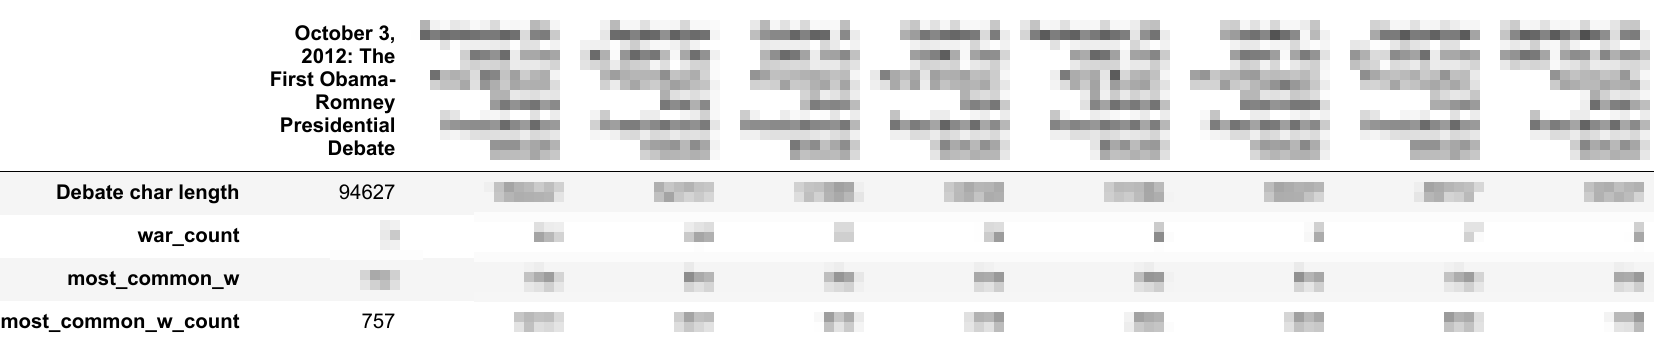
\includegraphics{https://github.com/ikhlaqsidhu/data-x/raw/master/x-archive/misc/hw2_imgs_spring2018/president_stats.png}
\caption{pres\_stats}
\end{figure}

\begin{center}\rule{0.5\linewidth}{\linethickness}\end{center}

.

    \subsection{2. Download and read in specific line from many data
sets}\label{download-and-read-in-specific-line-from-many-data-sets}

Scrape the first 27 data sets from this URL
http://people.sc.fsu.edu/\textasciitilde{}jburkardt/datasets/regression/
(i.e.\texttt{x01.txt} - \texttt{x27.txt}). Then, save the 5th line in
each data set, this should be the name of the data set author (get rid
of the \texttt{\#} symbol, the white spaces and the comma at the end).

Count how many times (with a Python function) each author is the
reference for one of the 27 data sets. Showcase your results, sorted,
with the most common author name first and how many times he appeared in
data sets. Use a Pandas DataFrame to show your results, see example.

\textbf{Example output of the answer EC Question 2:}

\begin{figure}
\centering
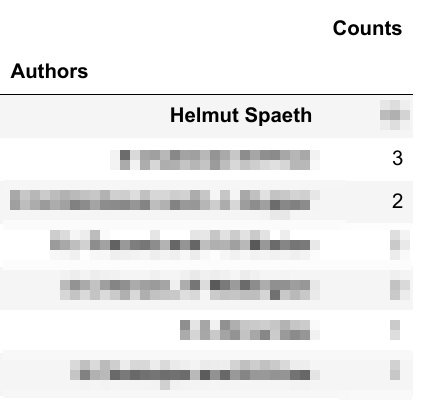
\includegraphics{https://github.com/ikhlaqsidhu/data-x/raw/master/x-archive/misc/hw2_imgs_spring2018/data_authors.png}
\caption{author\_stats}
\end{figure}


    % Add a bibliography block to the postdoc
    
    
    
    \end{document}
